%%%%%%%%%%%%%%%%%%%%%%%%%%%%%%%%%
% CHAPTER 2: Experimental Setup %
%%%%%%%%%%%%%%%%%%%%%%%%%%%%%%%%%

\renewcommand{\thechapter}{2}

\chapter{Experimental Setup}
\label{chap:exp_setup}
The series of field experiments described in this report were conducted in two structures of similar design located at the Delaware County Emergency Services Training Center in Sharon Hill, Pennsylvania. Three propane burners were used as the fire source for the experiments, and the structures were instrumented with various sensors to collect gas temperature, gas velocity, total heat flux, and gas species concentration measurements.

\section{Test Structures}
% The following sections contain detailed information about the construction of each experimental structure and the layout of the structures 

\subsection{Construction}
Each test structure was built on a concrete slab as shown in Figure~\ref{fig:struct_pics}. The East Structure and West Structure were designed to simulate a single-story and two-story residential structure, respectively.

\subsubsection*{\textit{First Floor of Both Structures}}
The first floor of each structure had outer walls composed of interlocking concrete blocks measuring 0.6~m (2.0~ft) wide, 0.6~m (2.0~ft) high, and 1.2~m (4.0~ft) long. The joints and gaps between the blocks were filled with high temperature insulation. All doors along the outer walls were composed of steel.

\begin{figure}
	\centering
	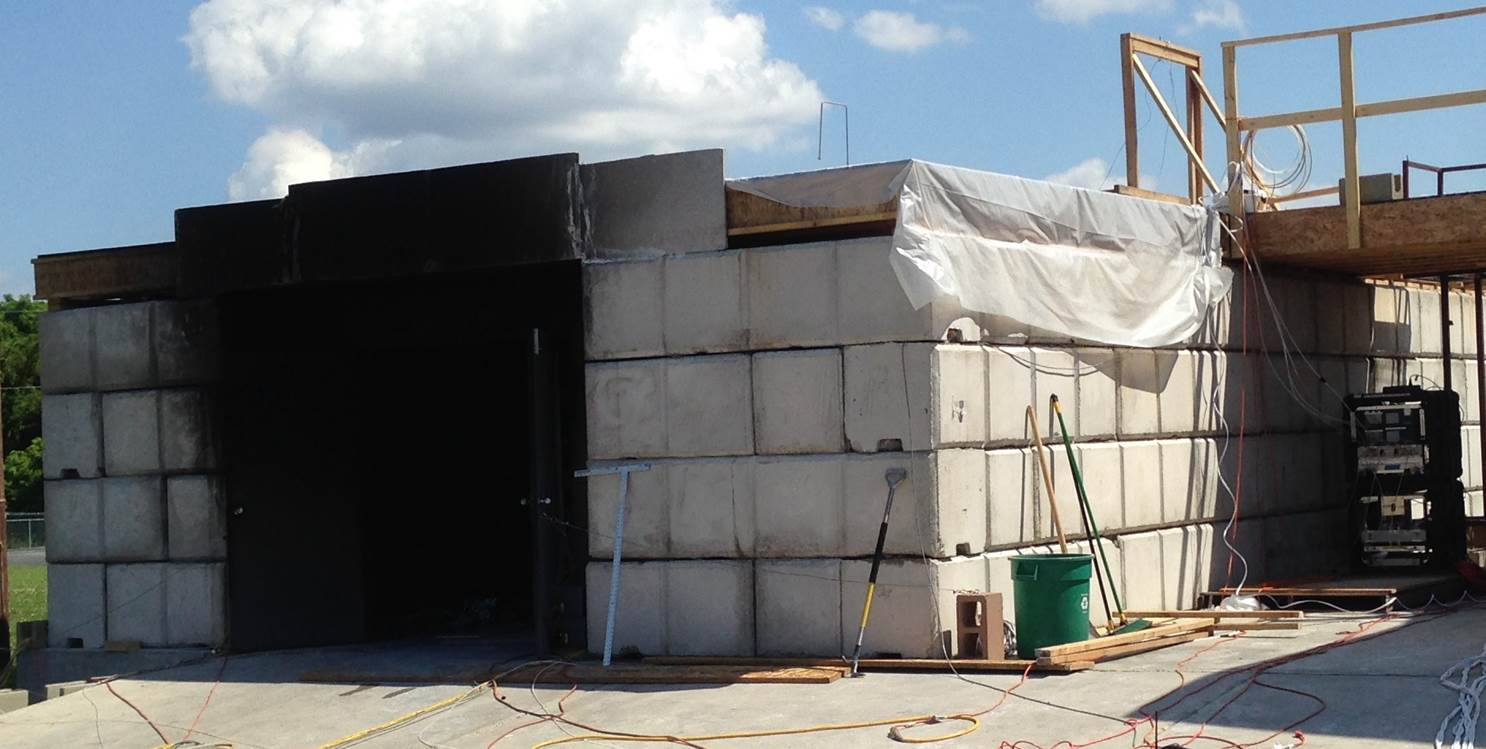
\includegraphics[width=5.25in]{Figures/Pictures/east_structure}
	\\~\\
	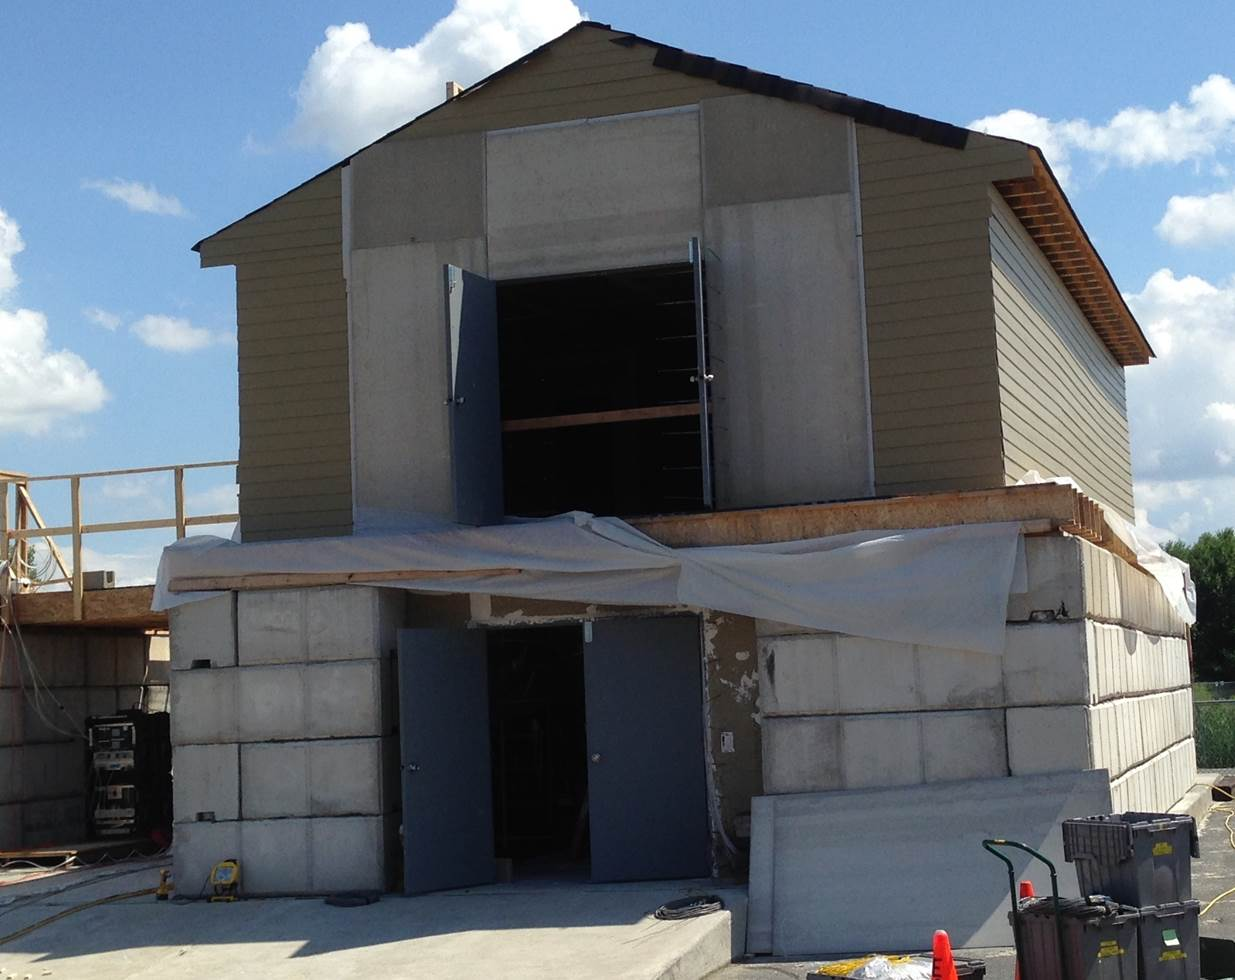
\includegraphics[width=5.25in]{Figures/Pictures/west_structure}
	\caption[North side of the East and West Structures]{North side of the East Structure (top) and West Structure (bottom).}
	\label{fig:struct_pics}
\end{figure}

The interior walls on the first floor of each structure were framed with steel studs set to 400~mm (16~in) centers and track. Two layers of 16~mm (0.63~in) Type X gypsum board lined the steel studs, and a layer of 13~mm (0.5~in) thick Durock cement board covered the gypsum board. The interior ceiling of each structure was covered by two layers of 13~mm (0.5~in) thick Durock cement board.

The first floor ceiling support of each structure was composed of wood truss joist I-beams (TJIs). Each TJI had a depth of 298~mm (11.75~in) and contained laminated veneer lumber flanges with a cross section of 29~mm (1.13~in) by 44~mm (1.75~in) and an 11~mm (0.43~in) thick oriented strand board (OSB) web as shown in Figure~\ref{fig:TJI}. A layer of 18.3~mm (0.72~in) thick tongue and groove OSB was attached to the top of the TJIs.

\begin{figure}[!h]
	\centering
	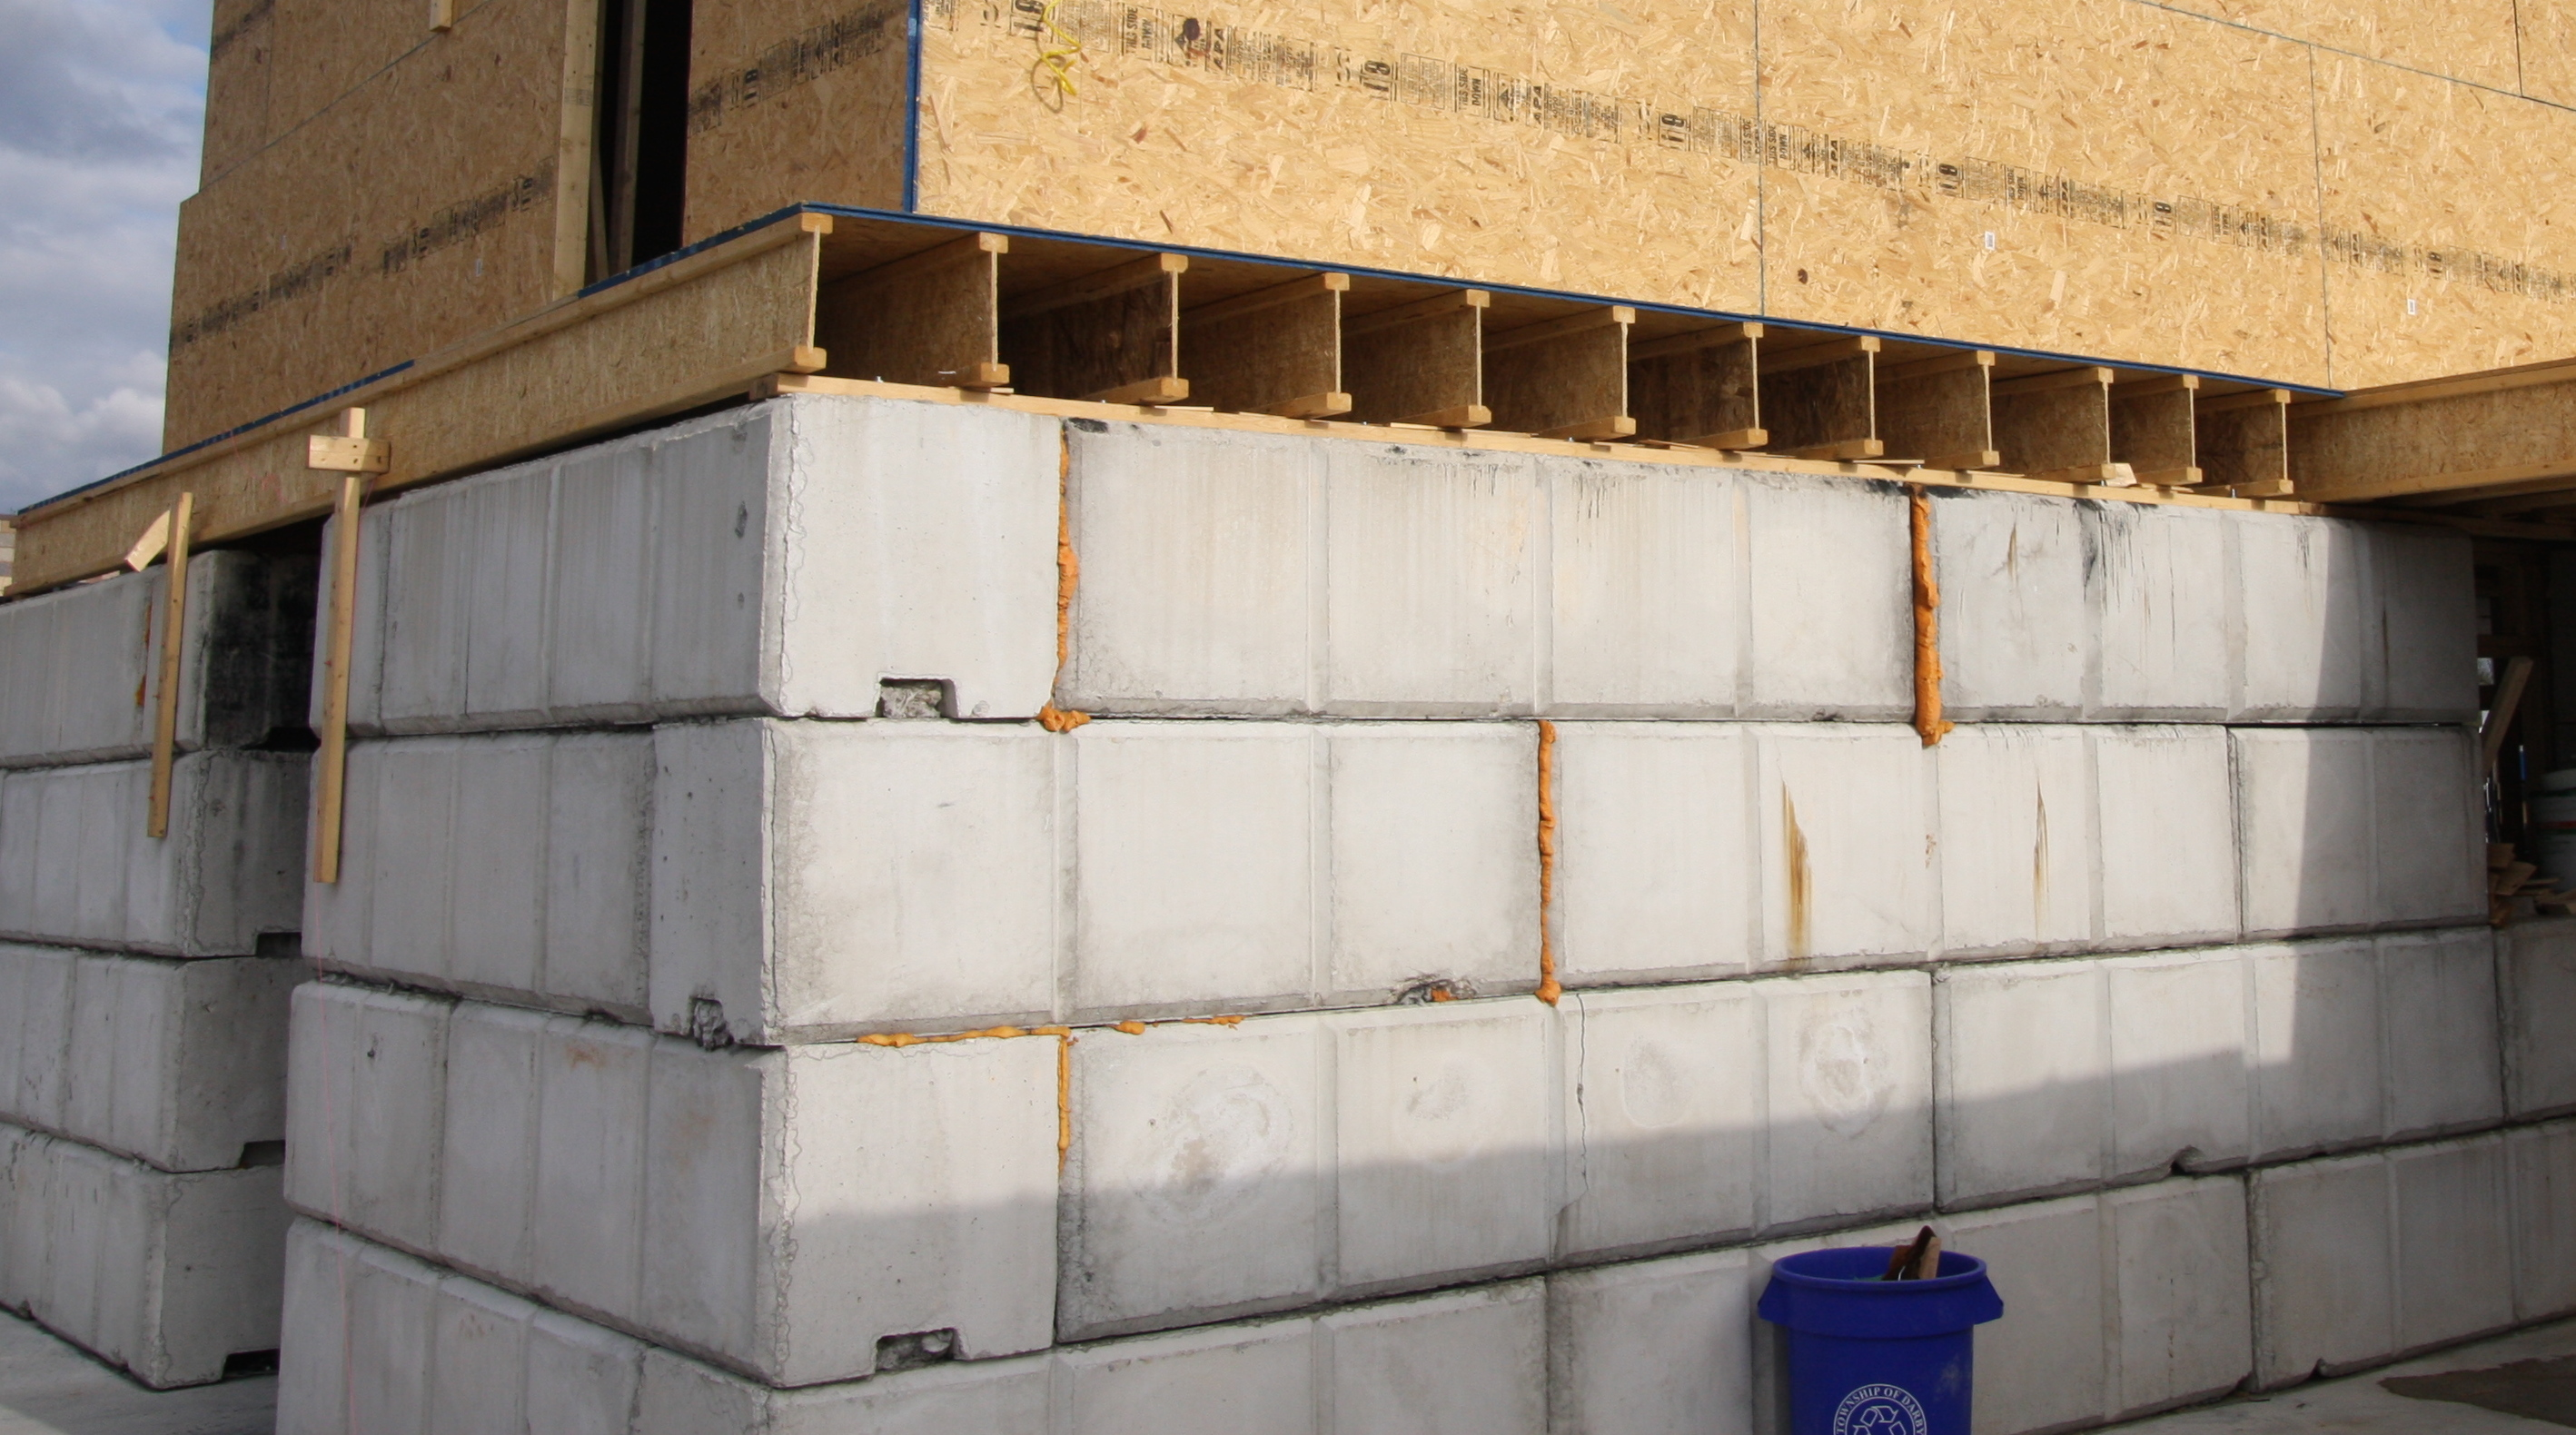
\includegraphics[width=0.9\columnwidth]{Figures/Pictures/TJI_support}
	\caption[Ceiling support of the West Structure]{First floor ceiling support of the West Structure composed of wood truss joist I-beams. View is of the southeast corner of the structure.}
	\label{fig:TJI}
\end{figure}
\FloatBarrier

\subsubsection*{\textit{Second Floor of West Structure}}
The second floor of the West Structure was built on the structure's first floor wood ceiling support. The two floors were connected by an interior stairwell. A door made of lauan plywood was located at the top of the stairwell. The walls on the second floor were wood frame with 51~mm (2~in) by 102~mm (4~in) studs set to 400~mm (16~in) centers. Two layers of 16~mm (0.63~in) Type X gypsum board lined the interior side of the wood studs, and a layer of 13~mm (0.5~in) thick Durock cement board covered the gypsum board. The interior ceiling of the second story was covered by two layers of 13~mm (0.5~in) thick Durock cement board. The exterior sides of the outer walls on the second floor were protected by 11~mm (0.44~in) thick OSB and 8~mm (0.31~in) fiber cement lap siding.

\subsection{Layout}
Dimensioned floor plans of the East and West Structures are presented in Figures~\ref{fig:east_dimensioned_plan}~and~\ref{fig:west_dimensioned_plan}, respectively.

\begin{figure}[!h]
	\centering
	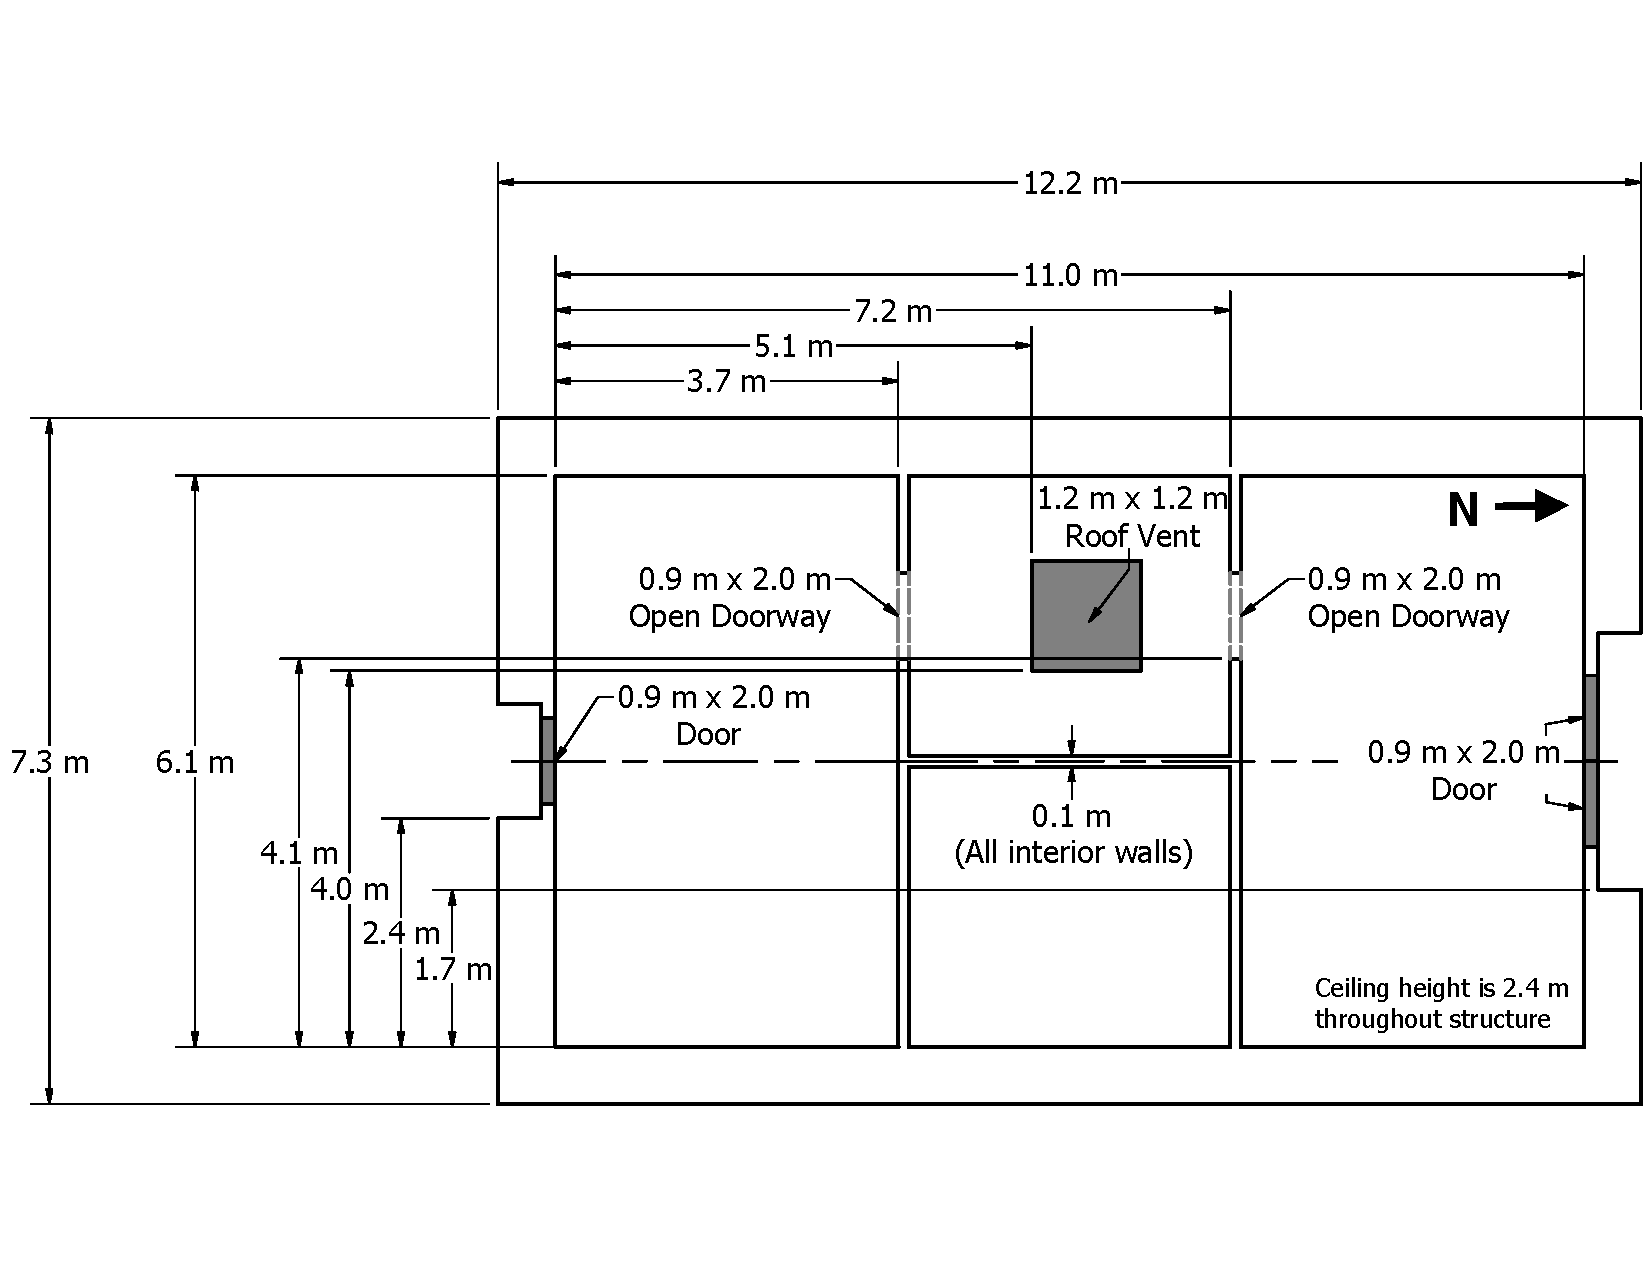
\includegraphics[width=\columnwidth]{Figures/Floor_Plans/East_Structure_Dimensioned_Full}
	\caption[Dimensioned floor plan of the East Structure]{Dimensioned floor plan of the East Structure. Structure dimensions are symmetric across horizontal centerline.}
	\label{fig:east_dimensioned_plan}
\end{figure}

\begin{figure}[!h]
	\centering
	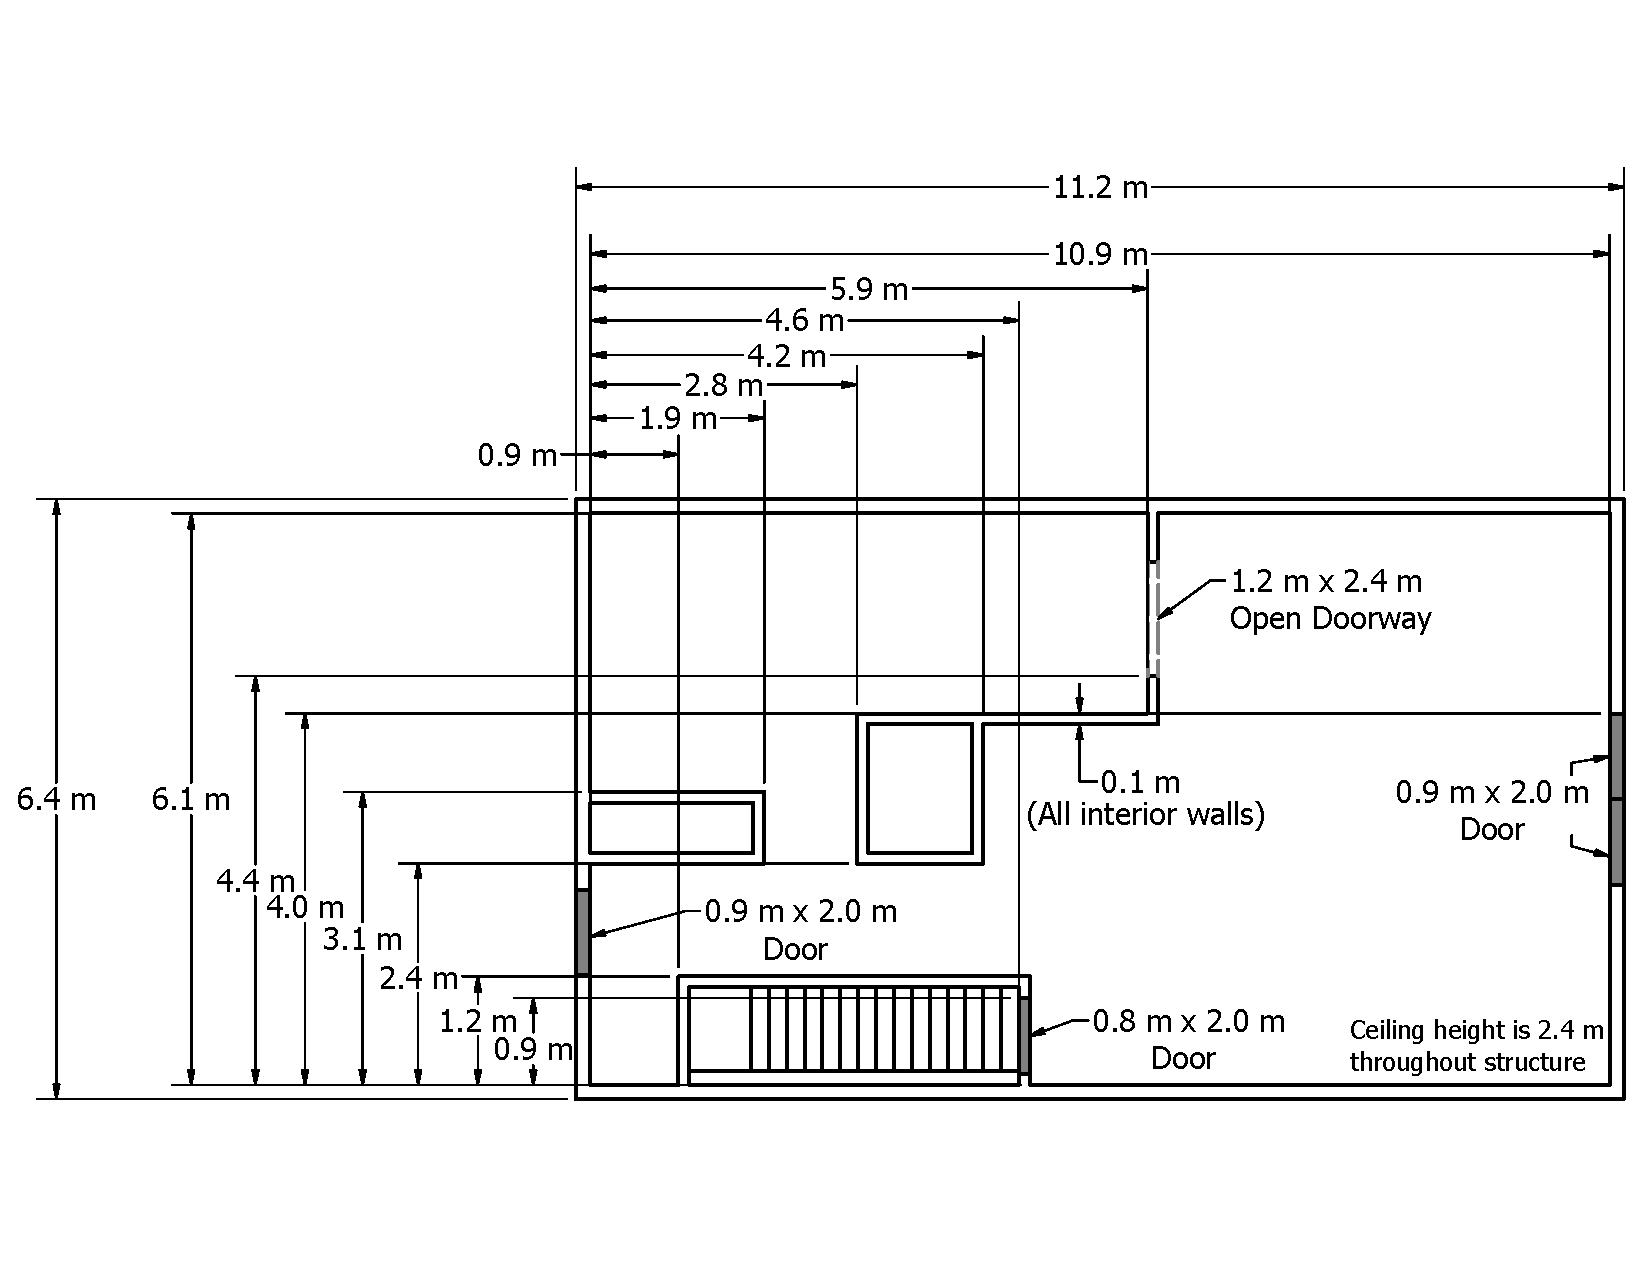
\includegraphics[width=\columnwidth]{Figures/Floor_Plans/West_Structure_2nd_Floor_Dimensioned_Full}
	\\~\\
	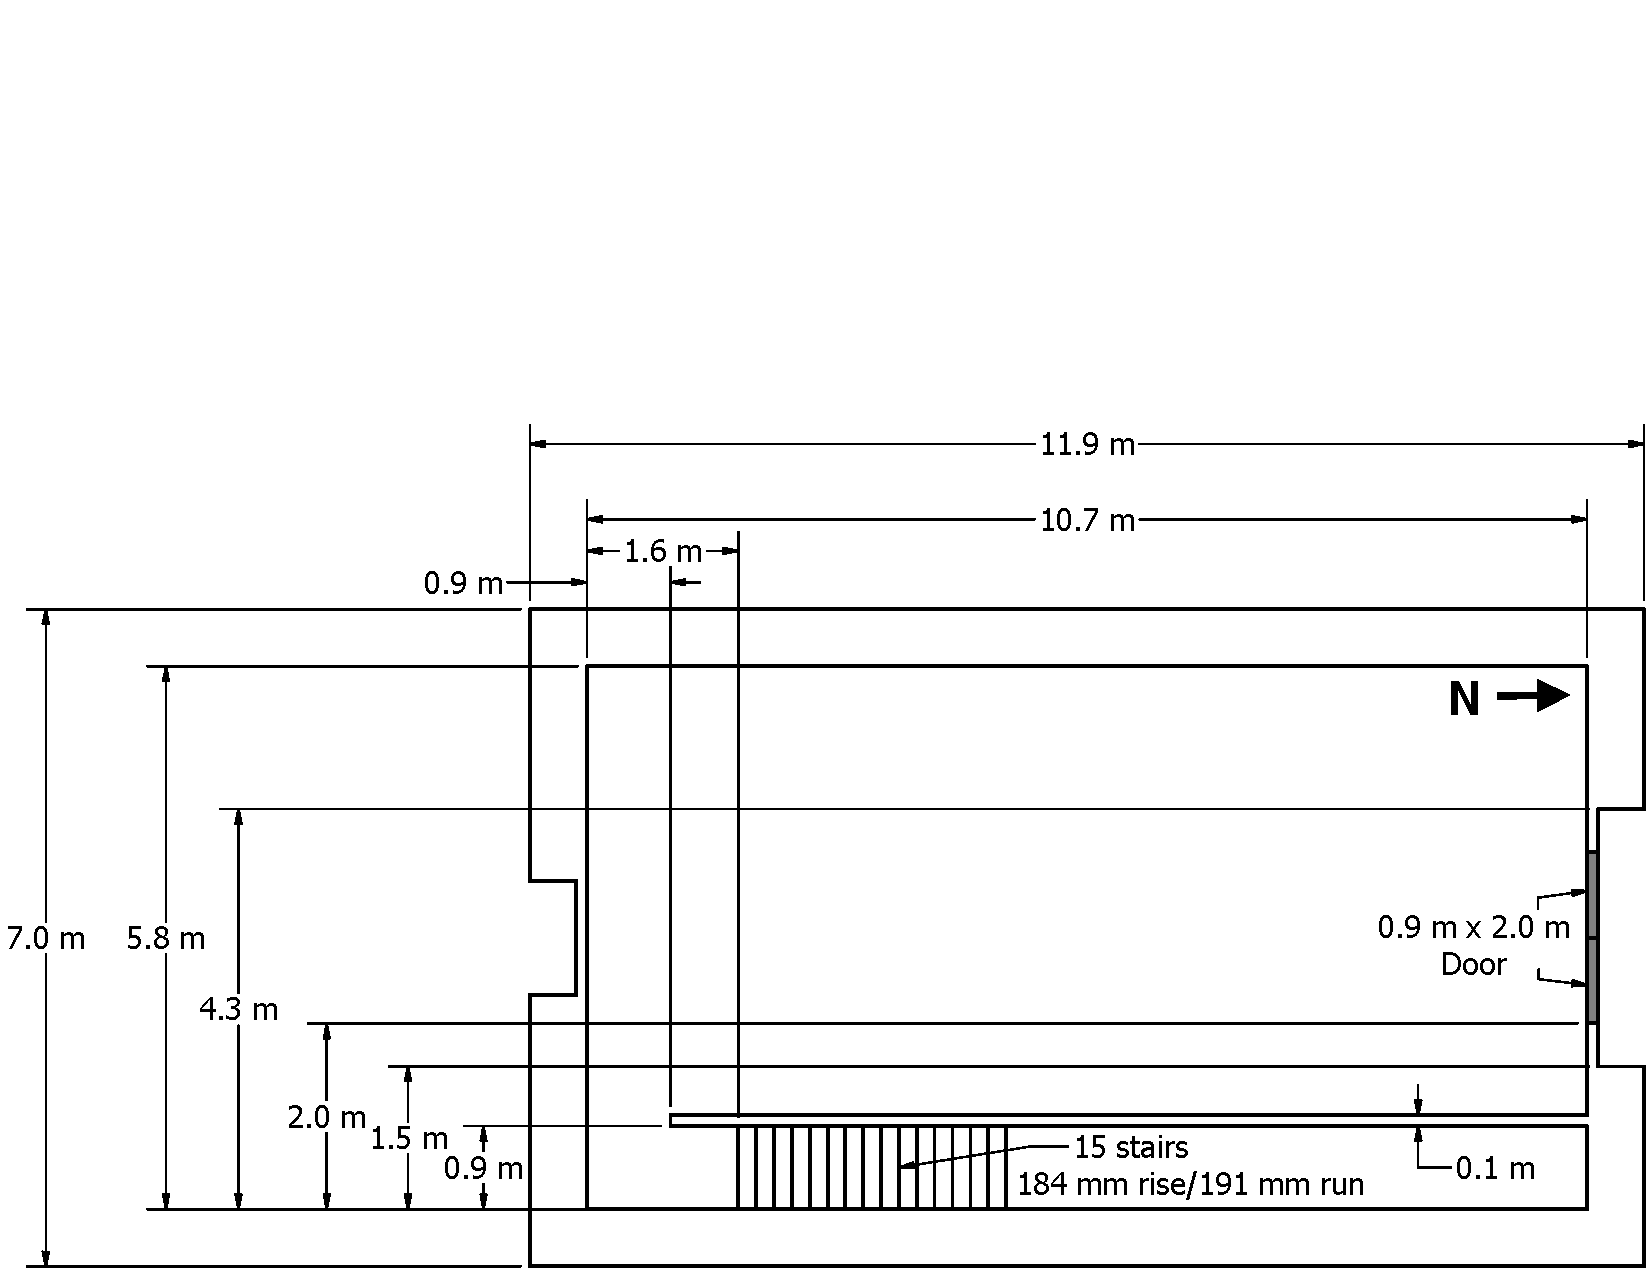
\includegraphics[width=\columnwidth]{Figures/Floor_Plans/West_Structure_1st_Floor_Dimensioned_Full}
	\caption[Dimensioned floor plans of the West Structure]{Dimensioned floor plan of the second floor (top) and first floor (bottom) of the West Structure.}
	\label{fig:west_dimensioned_plan}
\end{figure}
\clearpage
The exterior doors of both structures, the stairwell door in the West Structure, and the square roof vent with a depth of 320~mm (12.75~in) in the East Structure were opened and closed at certain instances during the experiments to change the ventilation within the structures.

\subsubsection*{\textit{Leakage}}
An air leakage measurement system~\cite{INFILTEC:leakage} from Infiltec, Inc. (model E3-A-DM4), was used to measure the amount of leakage associated with each structure. The amount of leakage in the East Structure was measured as 0.024~m$^2$. For the West Structure, the leakage was measured as 0.027~m$^2$ when the stairway door was fully closed, 0.054~m$^2$ when the stairway door was fully opened, and 0.048~m$^2$ when the stairway door was in the ``closed'' position (having a 152~mm (6~in) gap between the door and the frame) used during Tests~24 and 25.

\section{Instrumentation}
\label{sec:intrumentation}
The structures were instrumented for temperature, gas velocity, heat flux, and gas concentration measurements. Gas temperatures in the burn rooms were measured with bare-bead, Chromel-Alumel (type K) thermocouples. Additional single thermocouples were installed in conjunction with bi-directional probes for gas velocity measurements. The single thermocouples were bare-bead, Chromel-Alumel (type K) thermocouples with a 1.0~mm (0.04~in) nominal diameter. The thermocouple wire was protected with a 3.2~mm (0.13~in) diameter inconel sheath. Water-cooled Schmidt-Boelter gauges were used to measure the total heat flux at different locations throughout the structures. Calibrated pumps pulled gas samples through a sample conditioning system to eliminate moisture in the sample. Then, the dry gas samples were piped to a series of gas analyzers and the gas concentrations of oxygen and carbon dioxide were measured. A legend is presented in Figure~\ref{fig:Instrumentation_Legend} to clarify the instrumentation schematic diagrams presented in the follow sections.

\begin{figure}[!h]
	\centering
	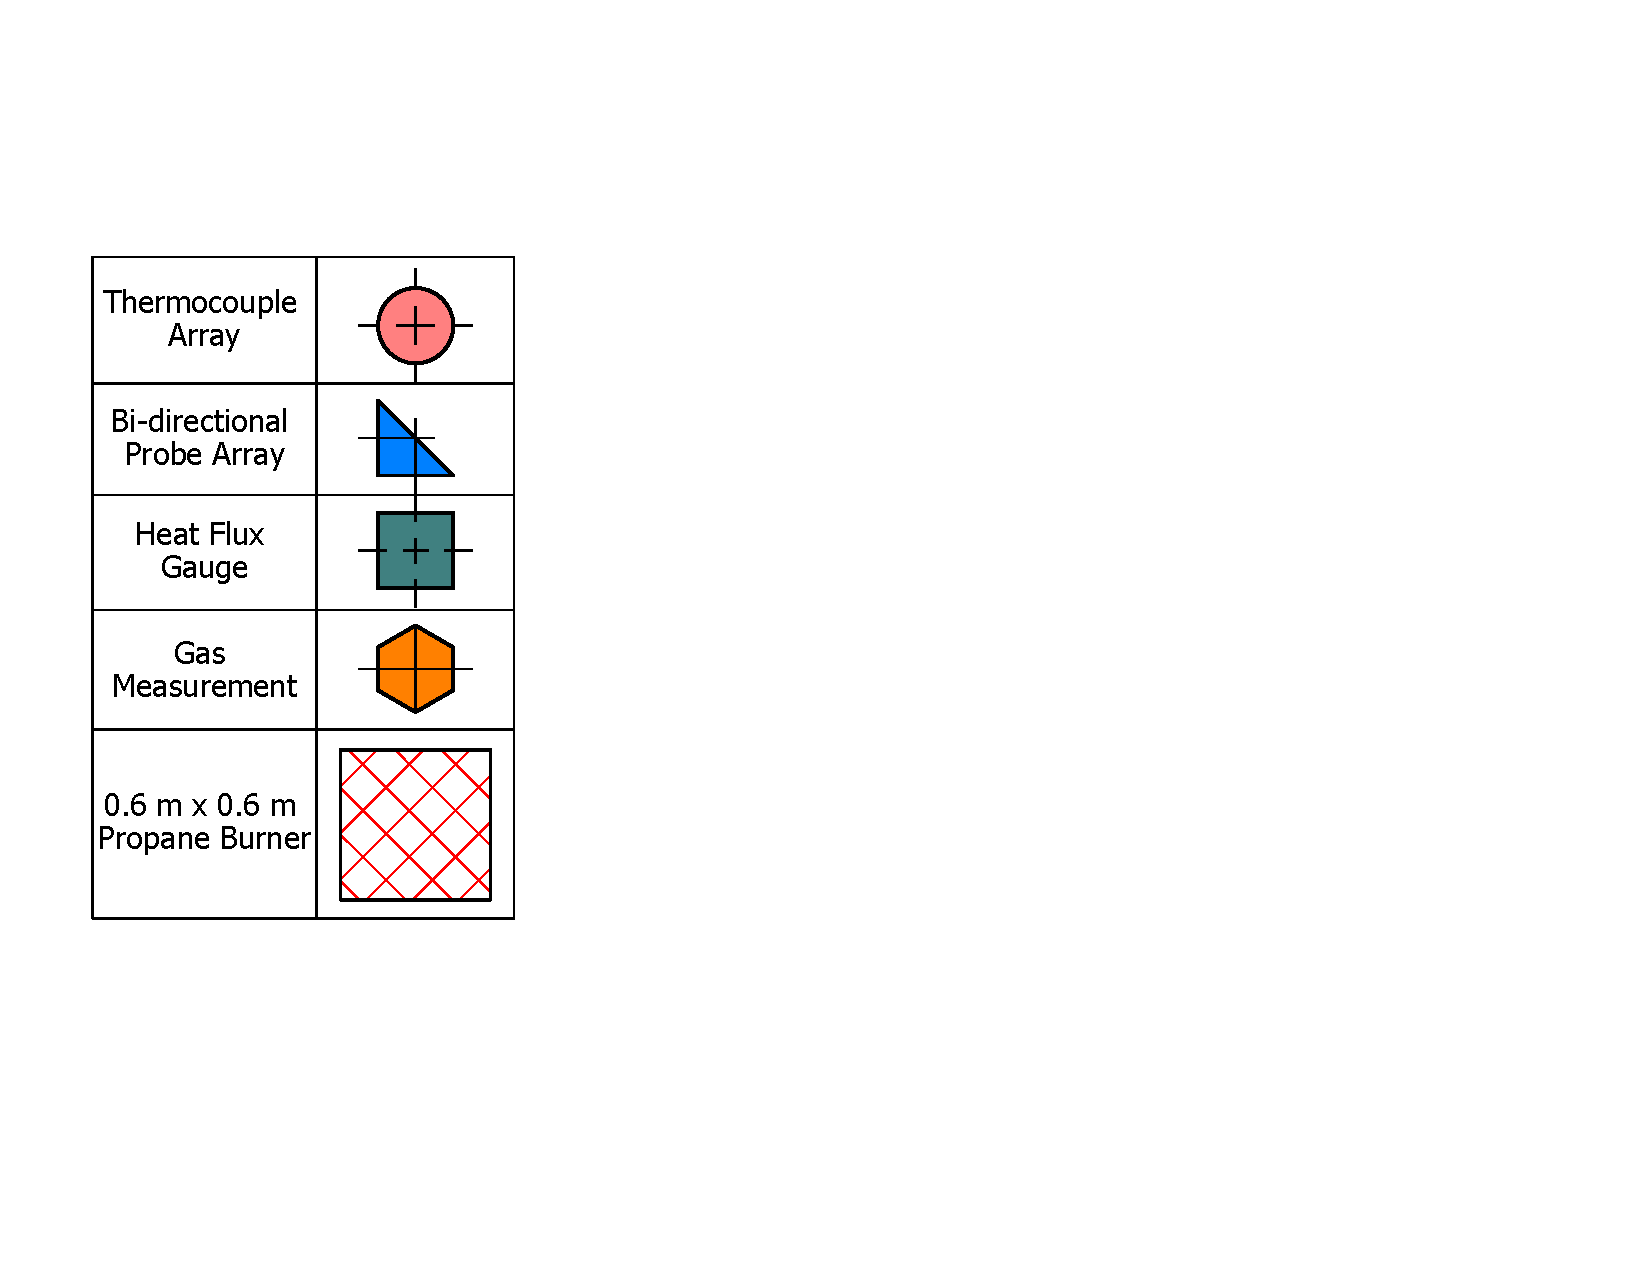
\includegraphics[width=0.25\columnwidth]{Figures/Floor_Plans/Instrumentation_Legend}
	% \begin{quote}
	\caption[Instrumentation legend]{Legend used for schematic diagrams of instrumentation locations.}
	% \end{quote}
	\label{fig:Instrumentation_Legend}
\end{figure}

Three diffusion flame burners, pictured in Figure~\ref{fig:burners}, were used as the fuel source for each experiment. Each burner had a square opening of side length 0.6~m (2~ft) located 0.14~m (5.5~in) above the floor and were positioned 0.6~m (2~ft) from the interior side of the south and west walls on the ground floor of each structure. Propane flowed from a supply truck to the gas burners for all experiments. The flow of propane to each burner was controlled by a high-precision turn valve, and the total displaced gas volume was measured using a rotary gas meter.

\begin{figure}[!h]
	\centering
	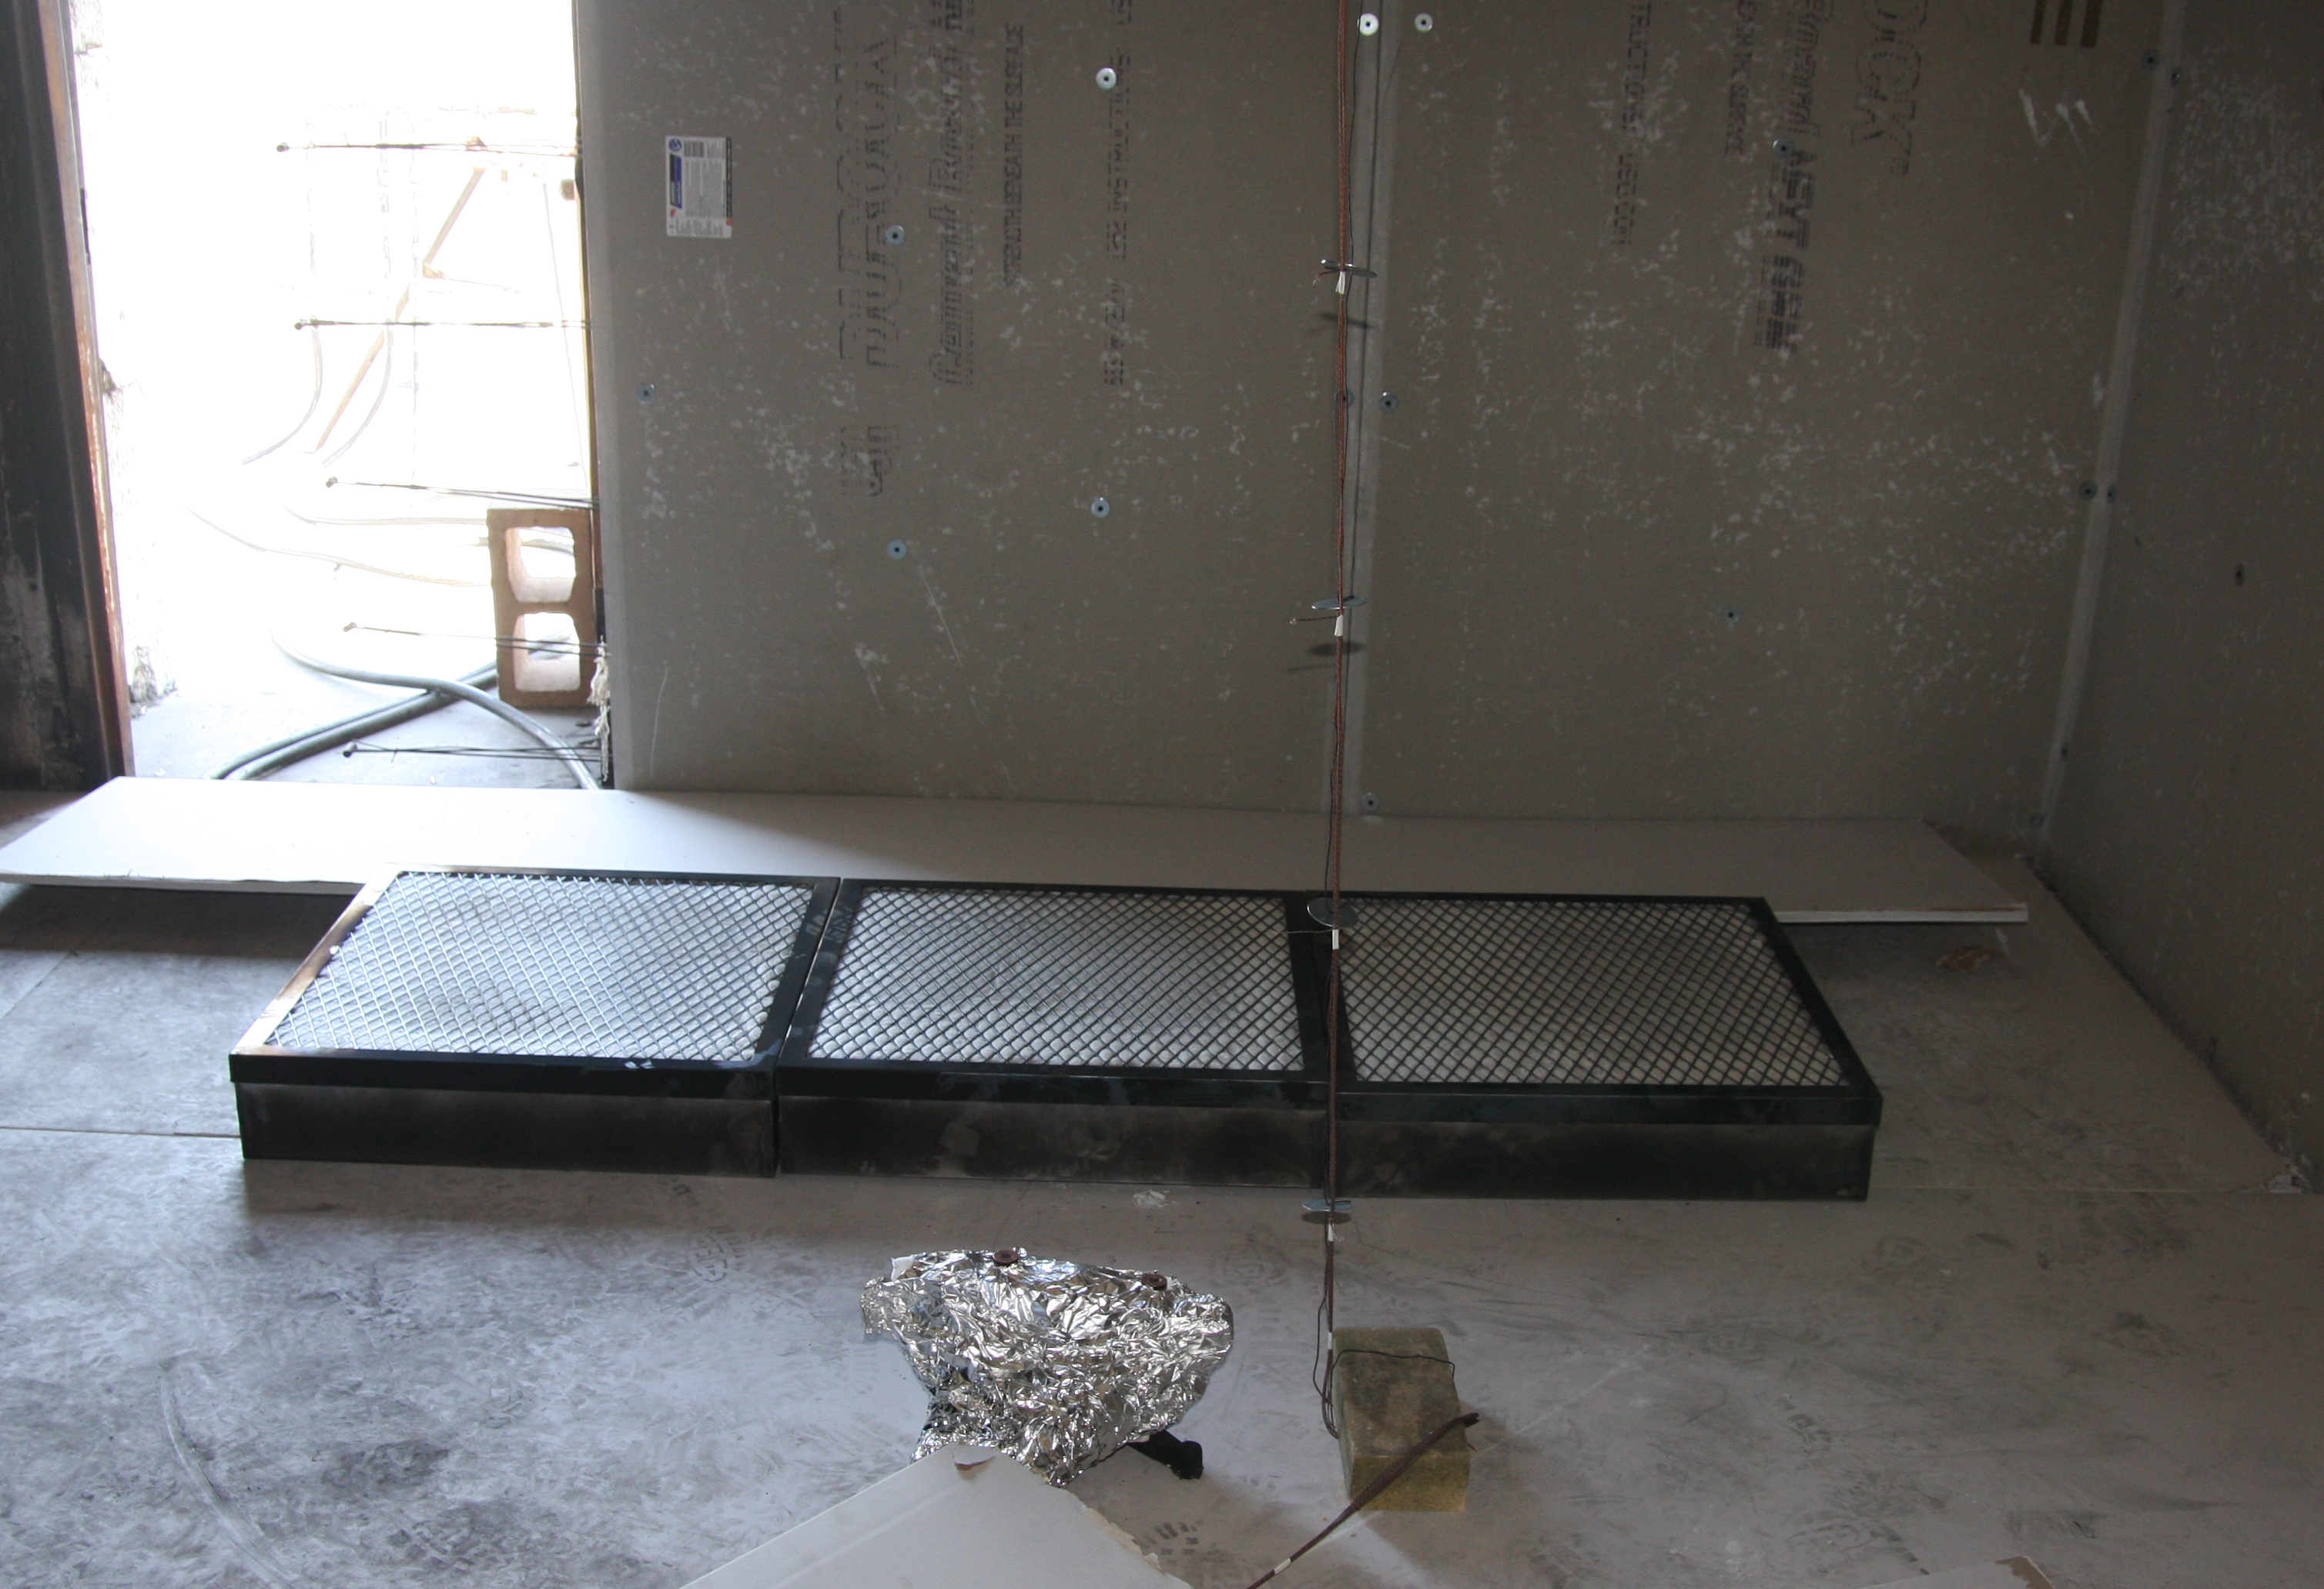
\includegraphics[width=0.9\columnwidth]{Figures/Pictures/burners}
	\caption[Three propane burners used as the fuel source.]{Three propane burners used as the fire source for the experiments located 0.6~m (2~ft) off the interior side of the south and west walls in the East Structure.}
	\label{fig:burners}
\end{figure}
\FloatBarrier

\subsection{East Structure}
The East Structure was instrumented with five bare-bead thermocouple arrays, four bi-directional probe plus solid thermocouple arrays, four total heat flux gauges, and two gas sample inlet pipes at the locations shown in Figure~\ref{fig:east_instrumentation}.

\begin{figure}[!h]
	\centering
	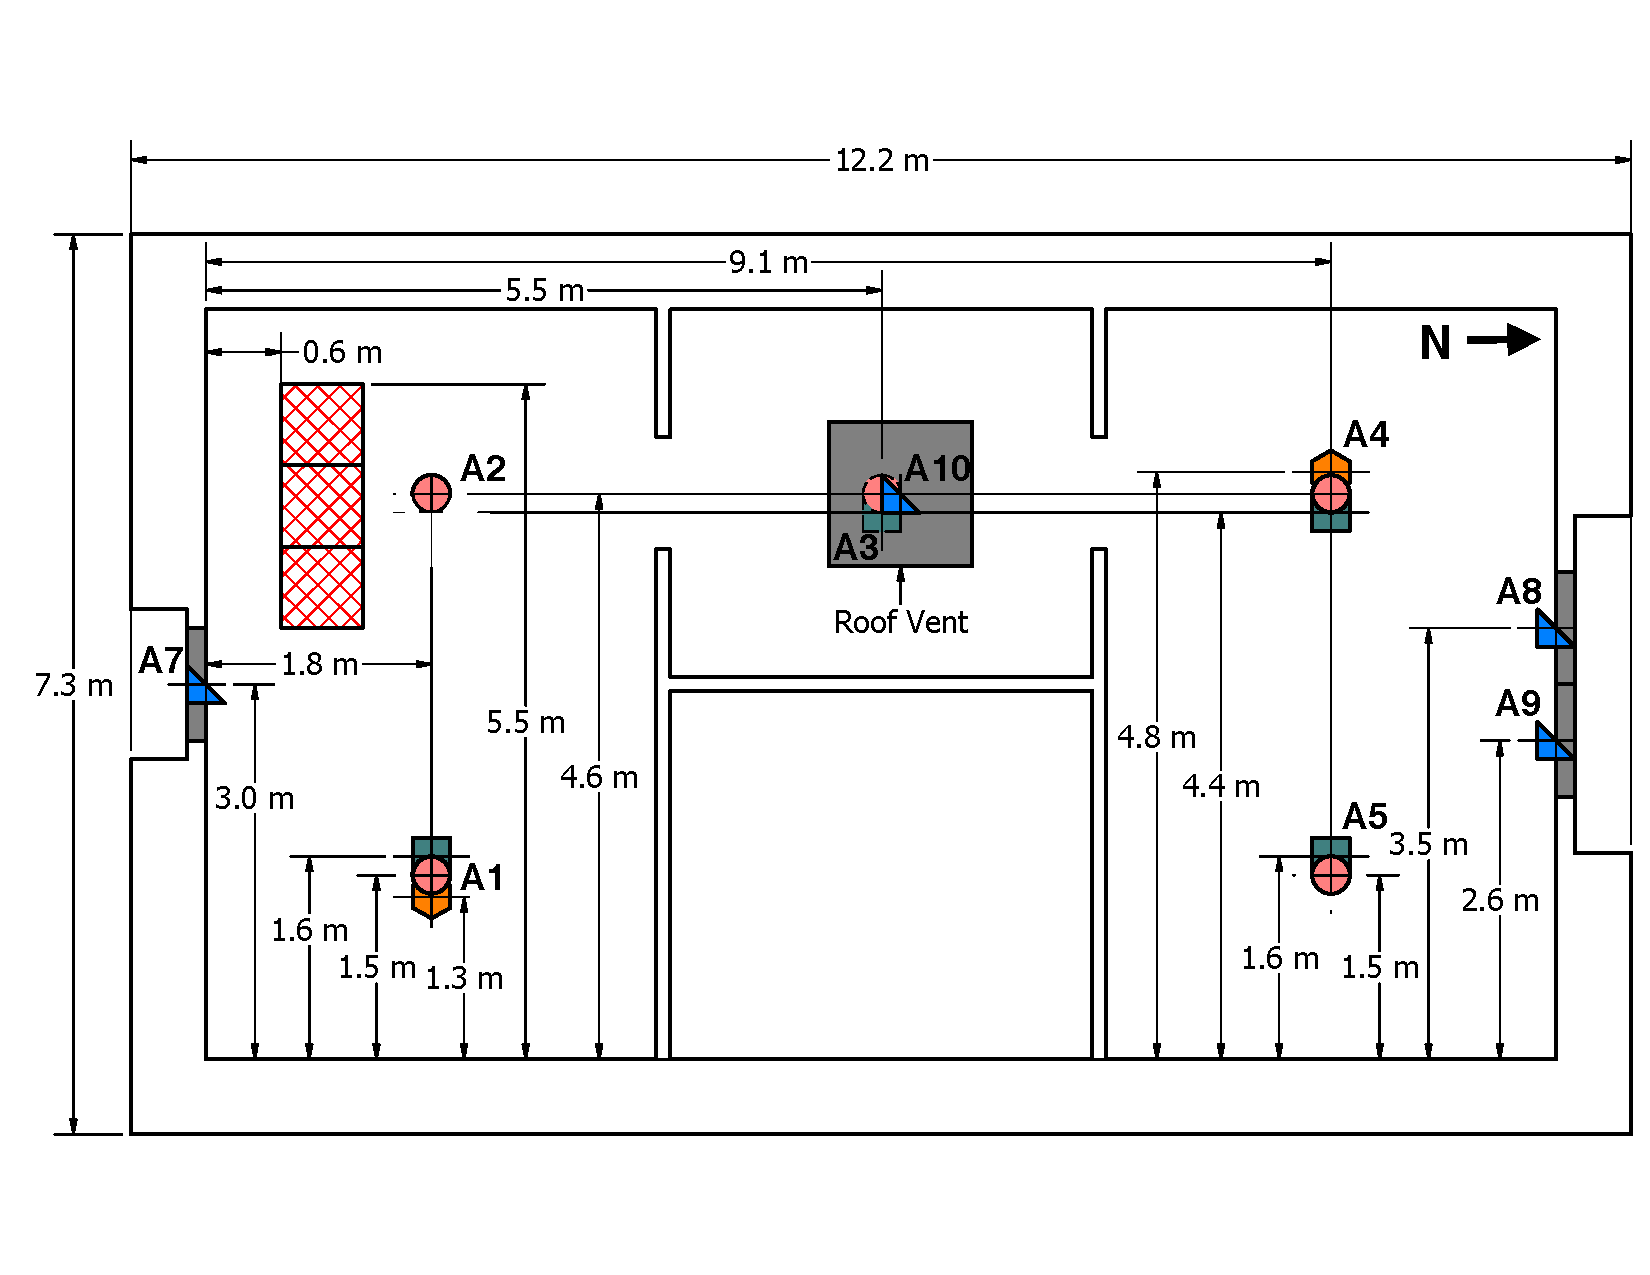
\includegraphics[width=\columnwidth]{Figures/Floor_Plans/East_Structure_Dimensioned_Instrumentation_New}
	\caption[Locations and labels of instrumentation in the East Structure]{Locations and labels of instrumentation in the East Structure.}
	\label{fig:east_instrumentation}
\end{figure}
\FloatBarrier

Each bare-bead thermocouple array (A1, A2, A3, A4, and A5) was composed of eight vertically-aligned thermocouples spaced between the floor and ceiling. Three bi-directional probe and solid thermocouple arrays (A7, A8, and A9) were centered in the exterior doorways of the structure and contained eight probes as shown in Figure~\ref{fig:BDP_arrays}. The fourth bi-directional probe and solid thermocouple array (A10), also presented in Figure~\ref{fig:BDP_arrays}, was located at the opening of the roof vent, 320~mm (12.75~in) above the compartment ceiling. The array contained three probes centered between the east and west sides of the vent. The position of each probe and thermocouple pair relative to the south wall of the vent is listed in Table~\ref{table:east_channel_list} of Appendix~\ref{chap:channel_lists}. The total heat flux gauges (A1, A3, A4, and A5) were located near the floor and aimed to view the ceiling. Lastly, gas samples were pulled from the environment through 9.5~mm (0.38~in) diameter stainless steel tubing (A1 and A4). The height of each individual sensor in the sensor arrays is listed in Table~\ref{table:east_channel_list} of Appendix~\ref{chap:channel_lists}.

\begin{figure}[!h]
	\centering
	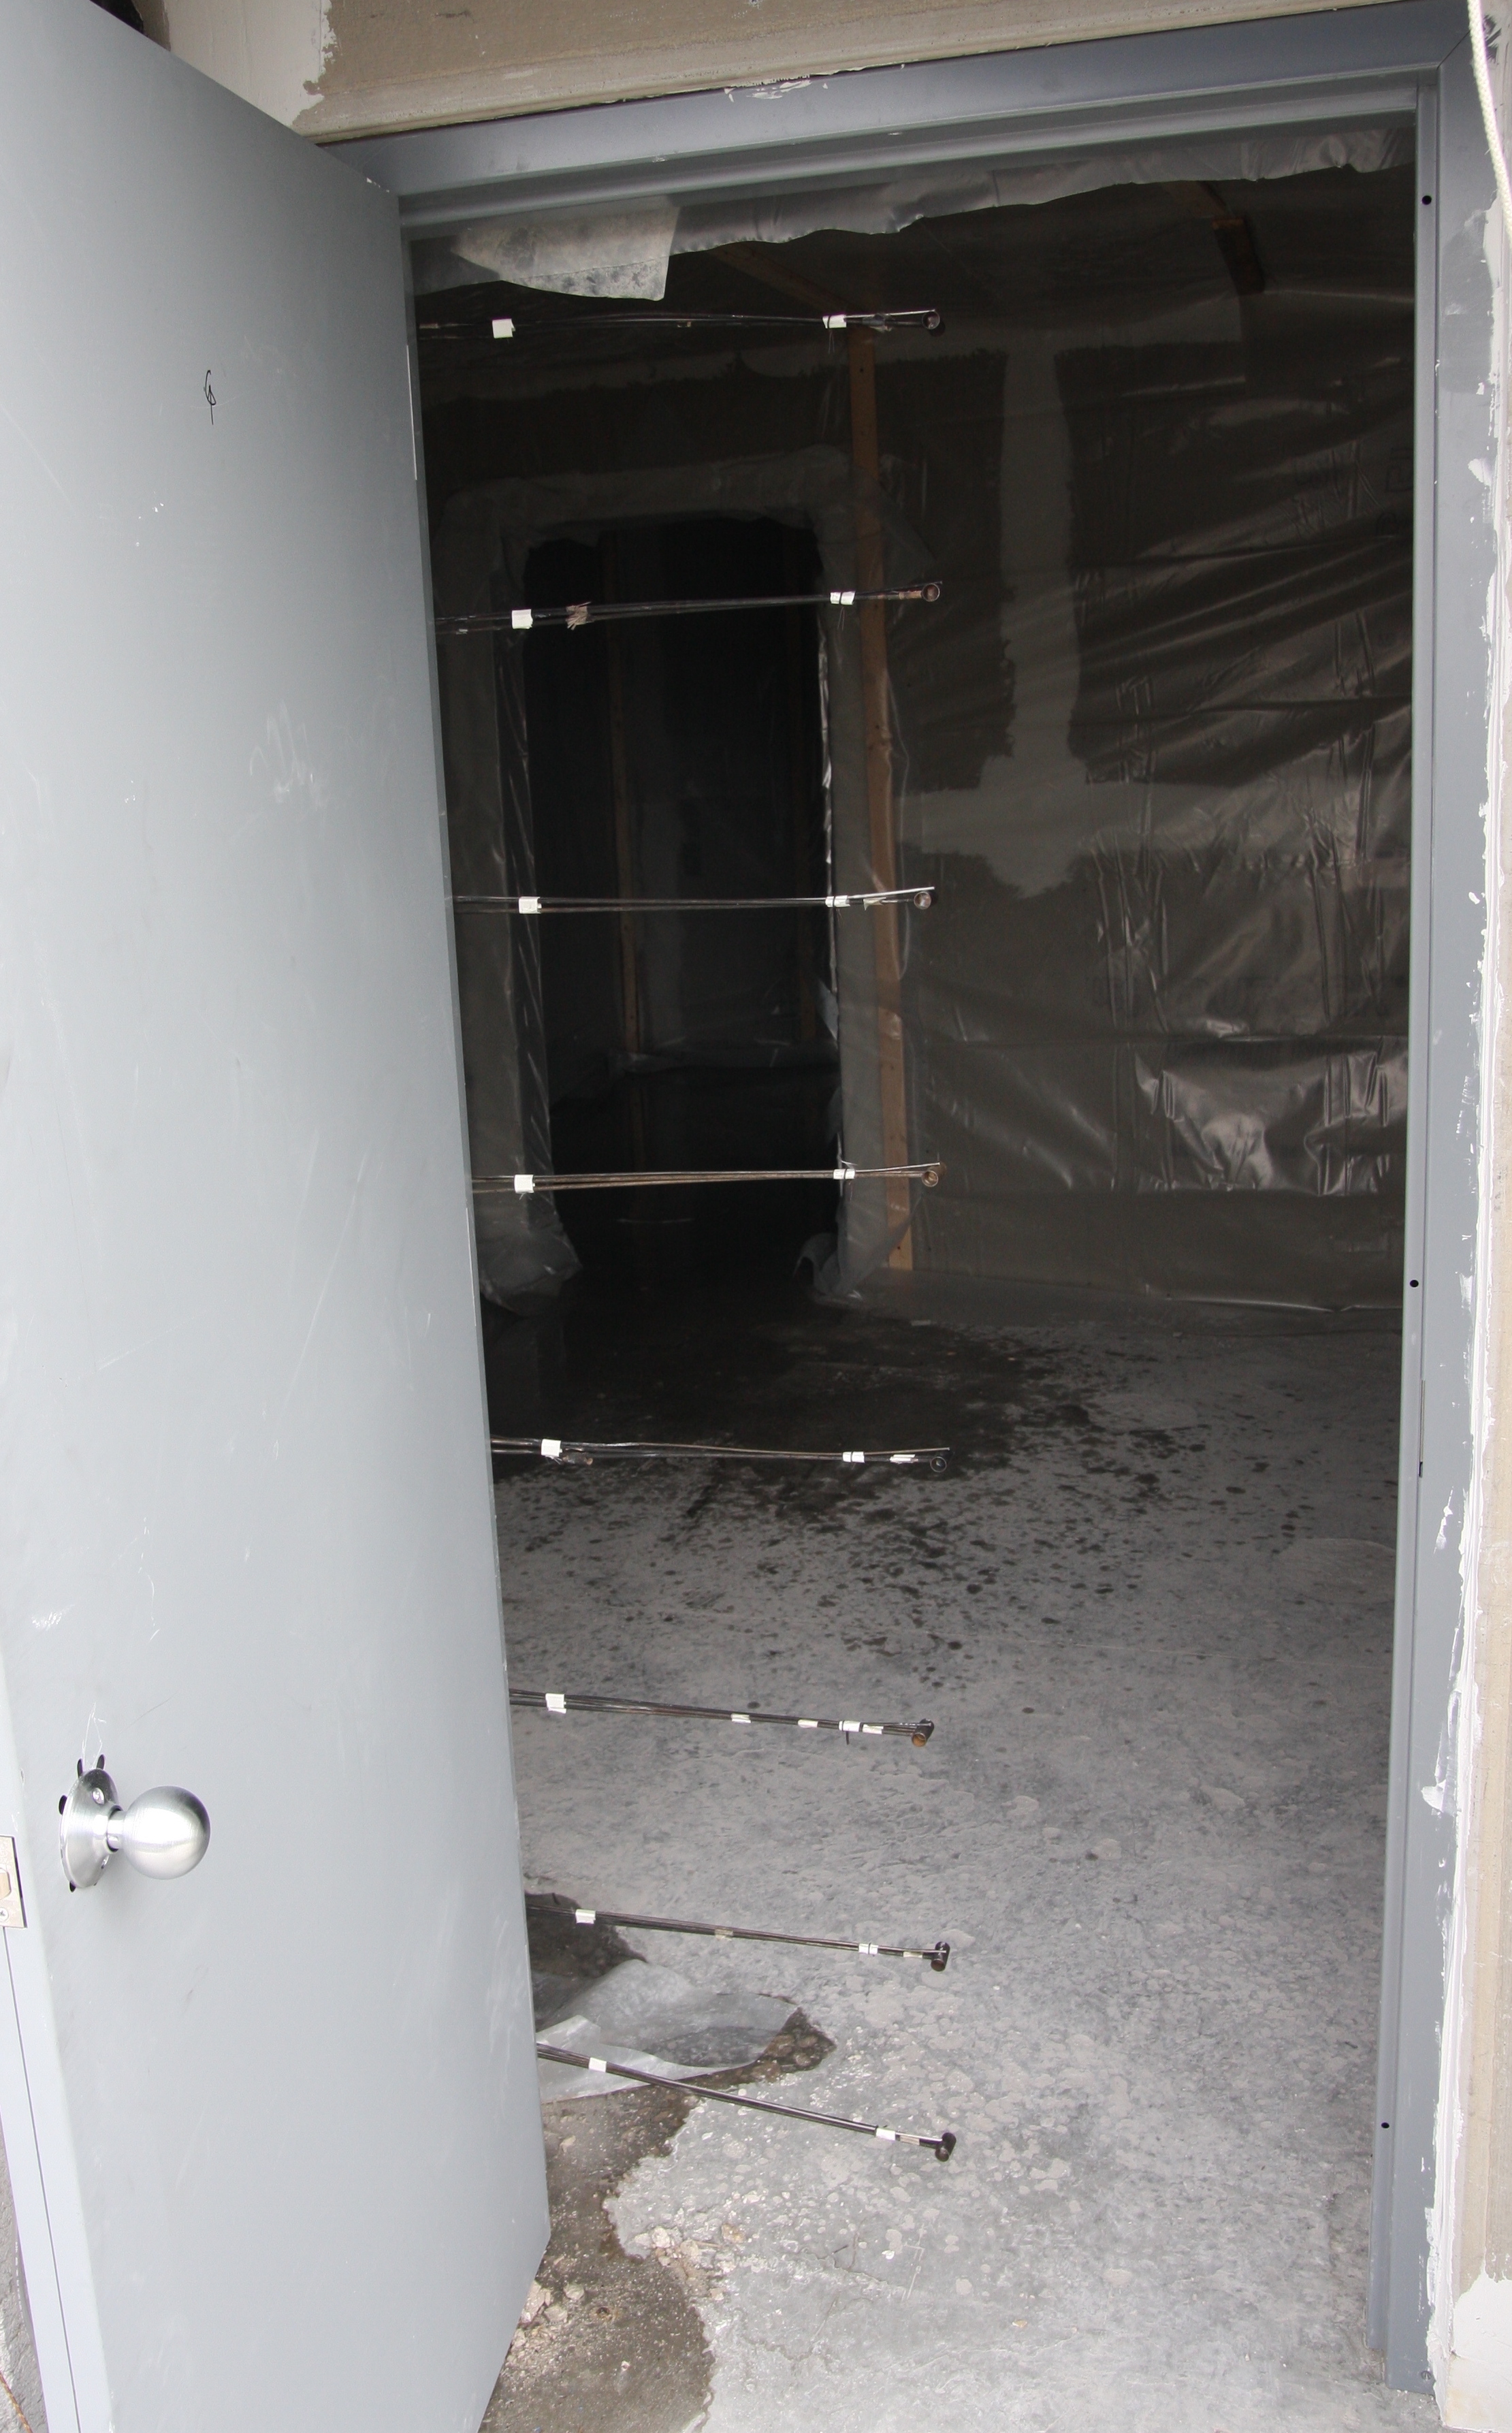
\includegraphics[width=0.35\columnwidth]{Figures/Pictures/doorway_BDPs}
	\\~\\
	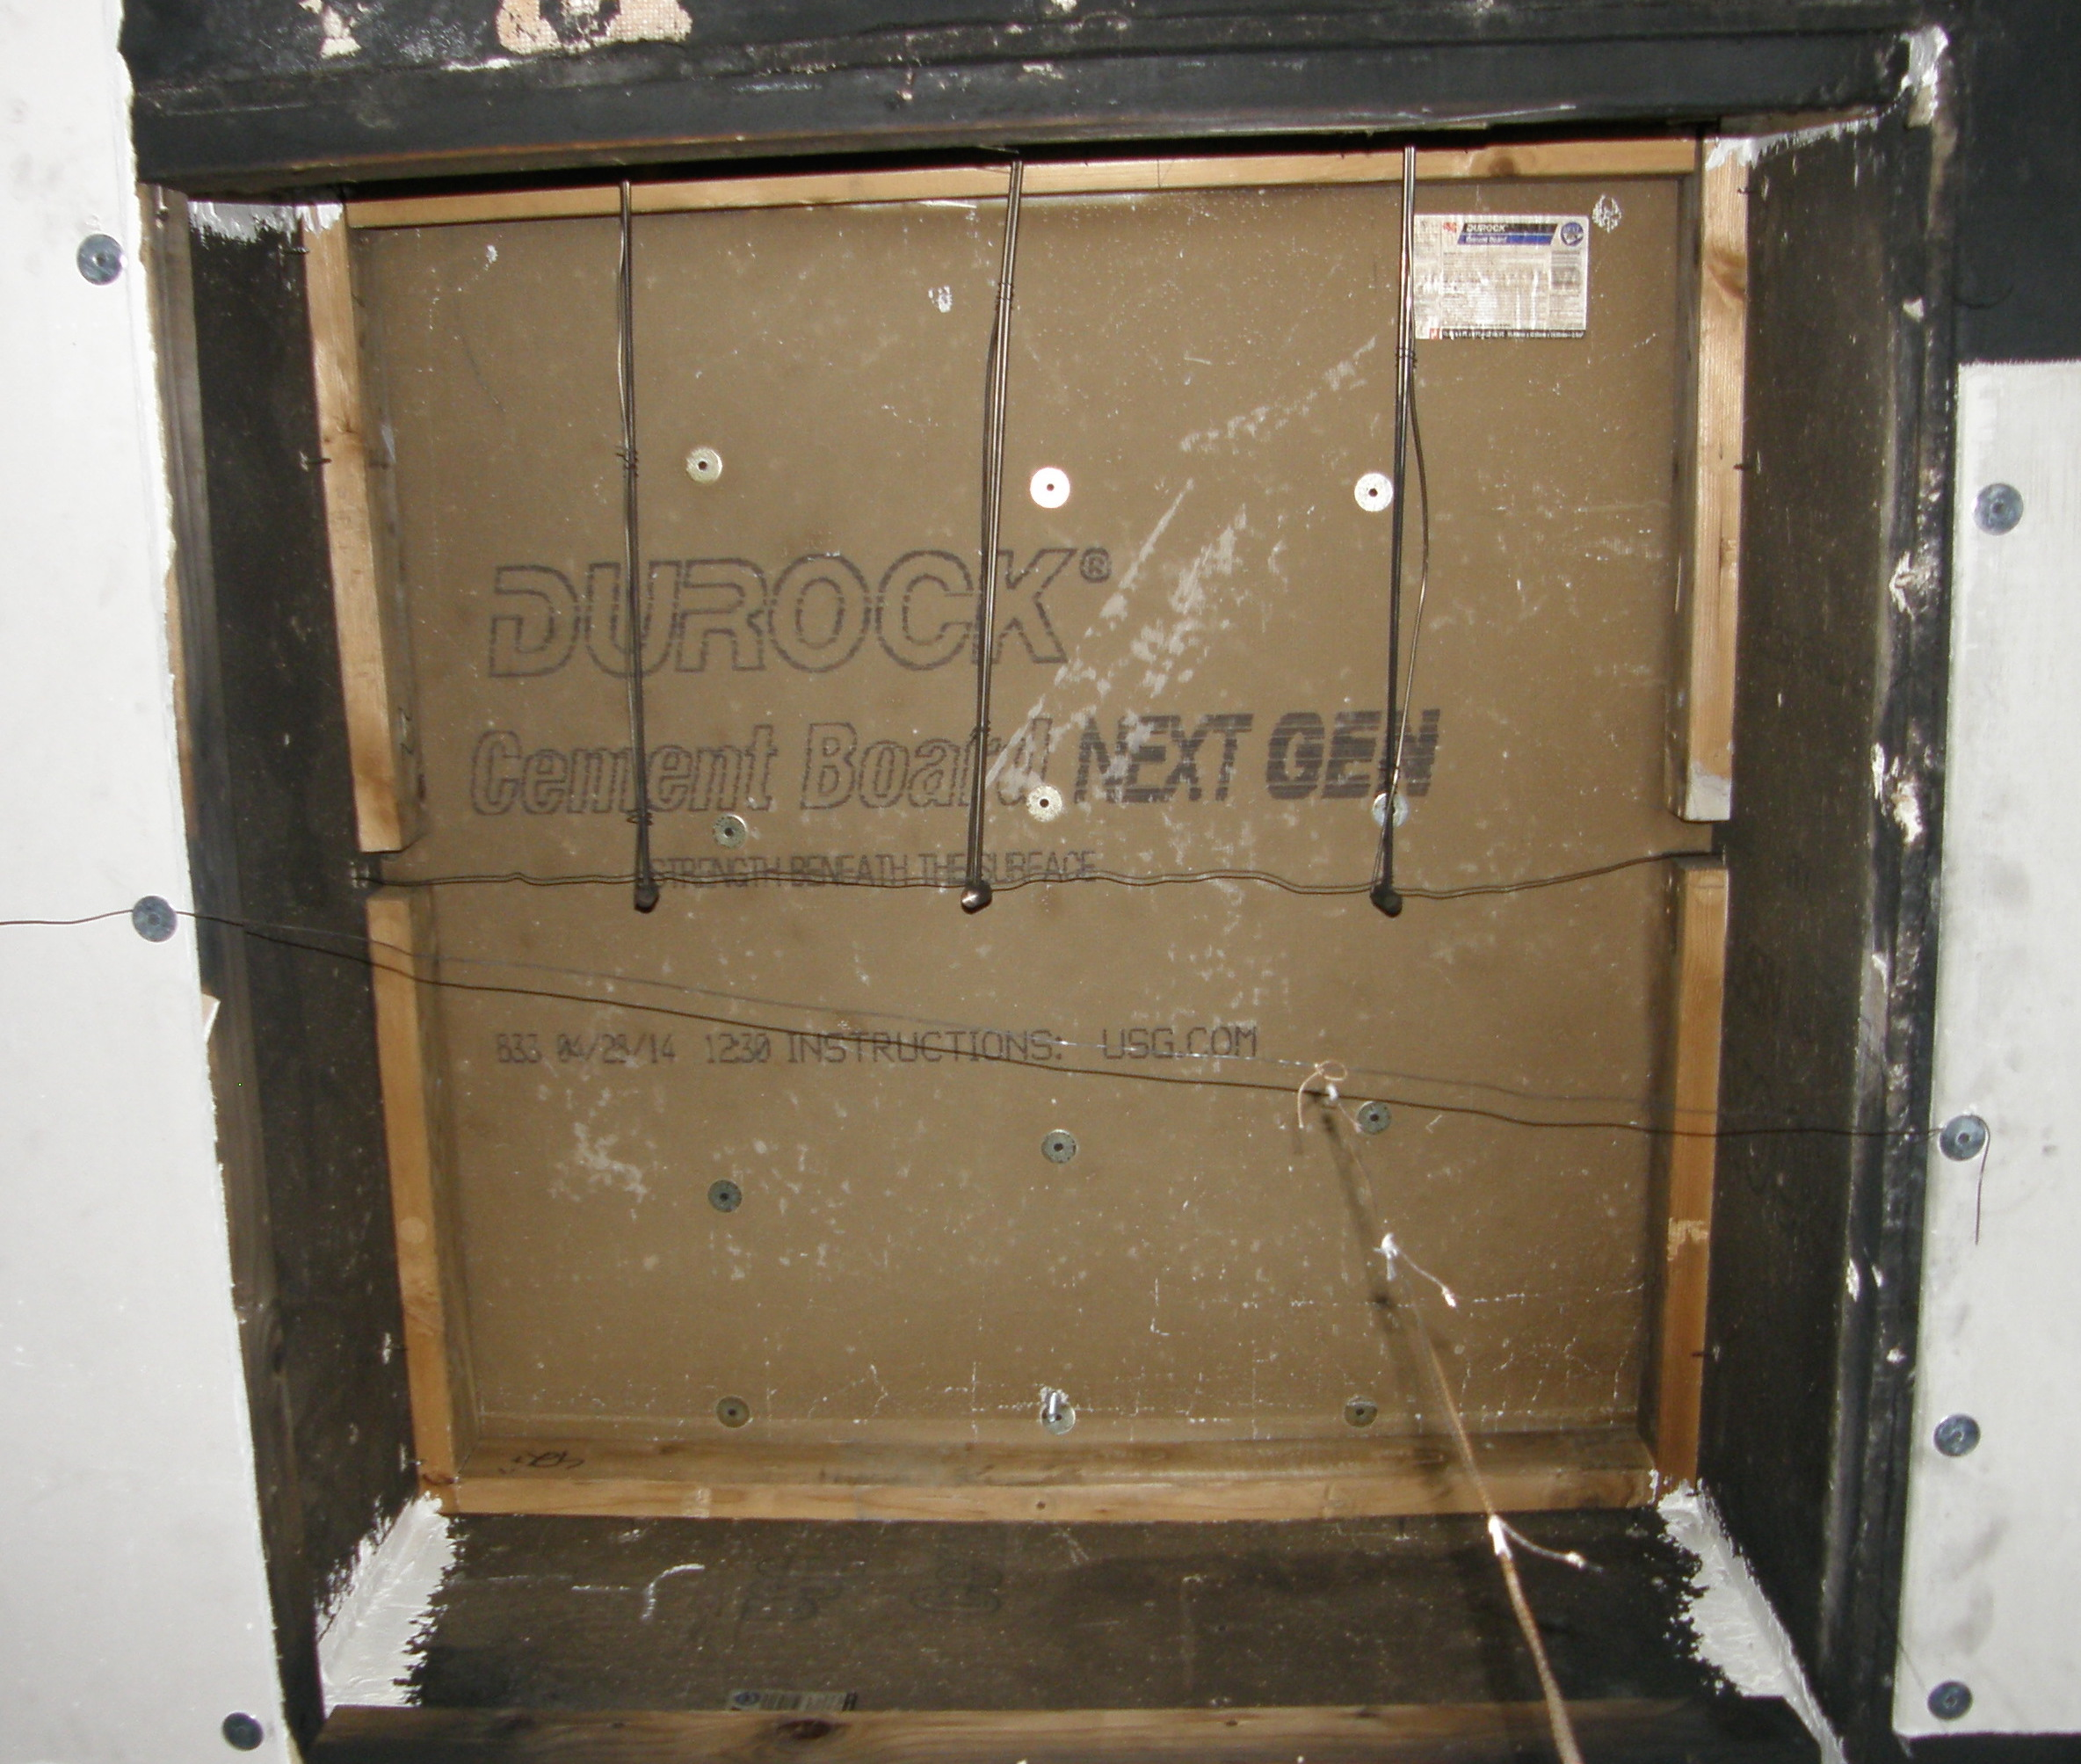
\includegraphics[width=0.55\columnwidth]{Figures/Pictures/roof_vent_BDPs}
	\caption[Bi-directional probe plus solid thermocouple arrays in East Structure]{Bi-directional probe plus solid thermocouple array at the south exterior doorway (top) and roof vent (bottom) of the East Structure.}
	\label{fig:BDP_arrays}
\end{figure}
\FloatBarrier

\subsection{West Structure}
The first floor of the West Structure was instrumented with three bare-bead thermocouple arrays (A1, A2, and A3), two bi-directional probe plus solid thermocouple arrays (A5 and A6), and one gas sample inlet pipe (A1). The second floor was equipped with three bare-bead thermocouple arrays (A7, A8, and A9), four bi-directional probe plus solid thermocouple arrays (A10, A11, A13, and A14), two total heat flux sensor pairs (A16 and A17), and one gas sample inlet pipe (A10). The location of the instrumentation in the West Structure is shown in Figure~\ref{fig:west_instrumentation}.

\begin{figure}[!ht]
	\centering
	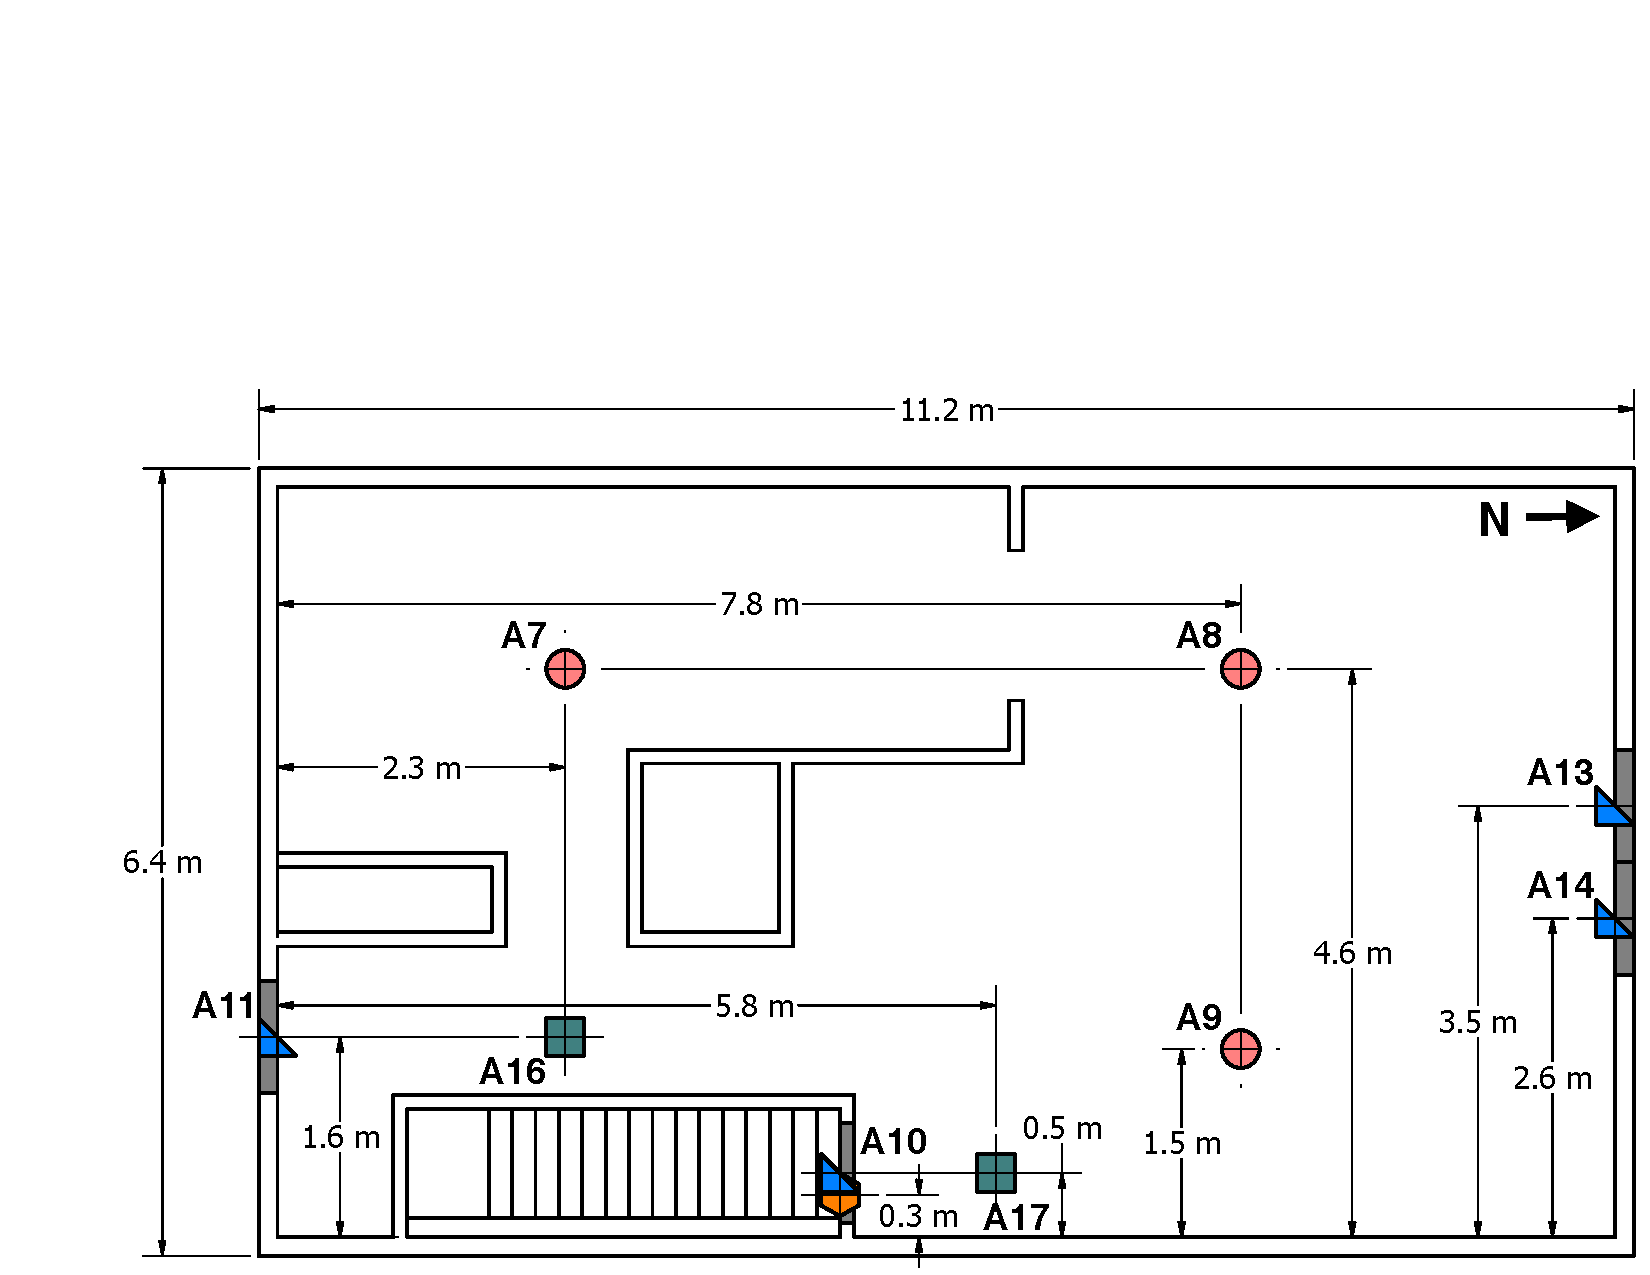
\includegraphics[width=0.94\columnwidth]{Figures/Floor_Plans/West_Structure_2nd_Floor_Dimensioned_Instrumentation}
	\\~\\
	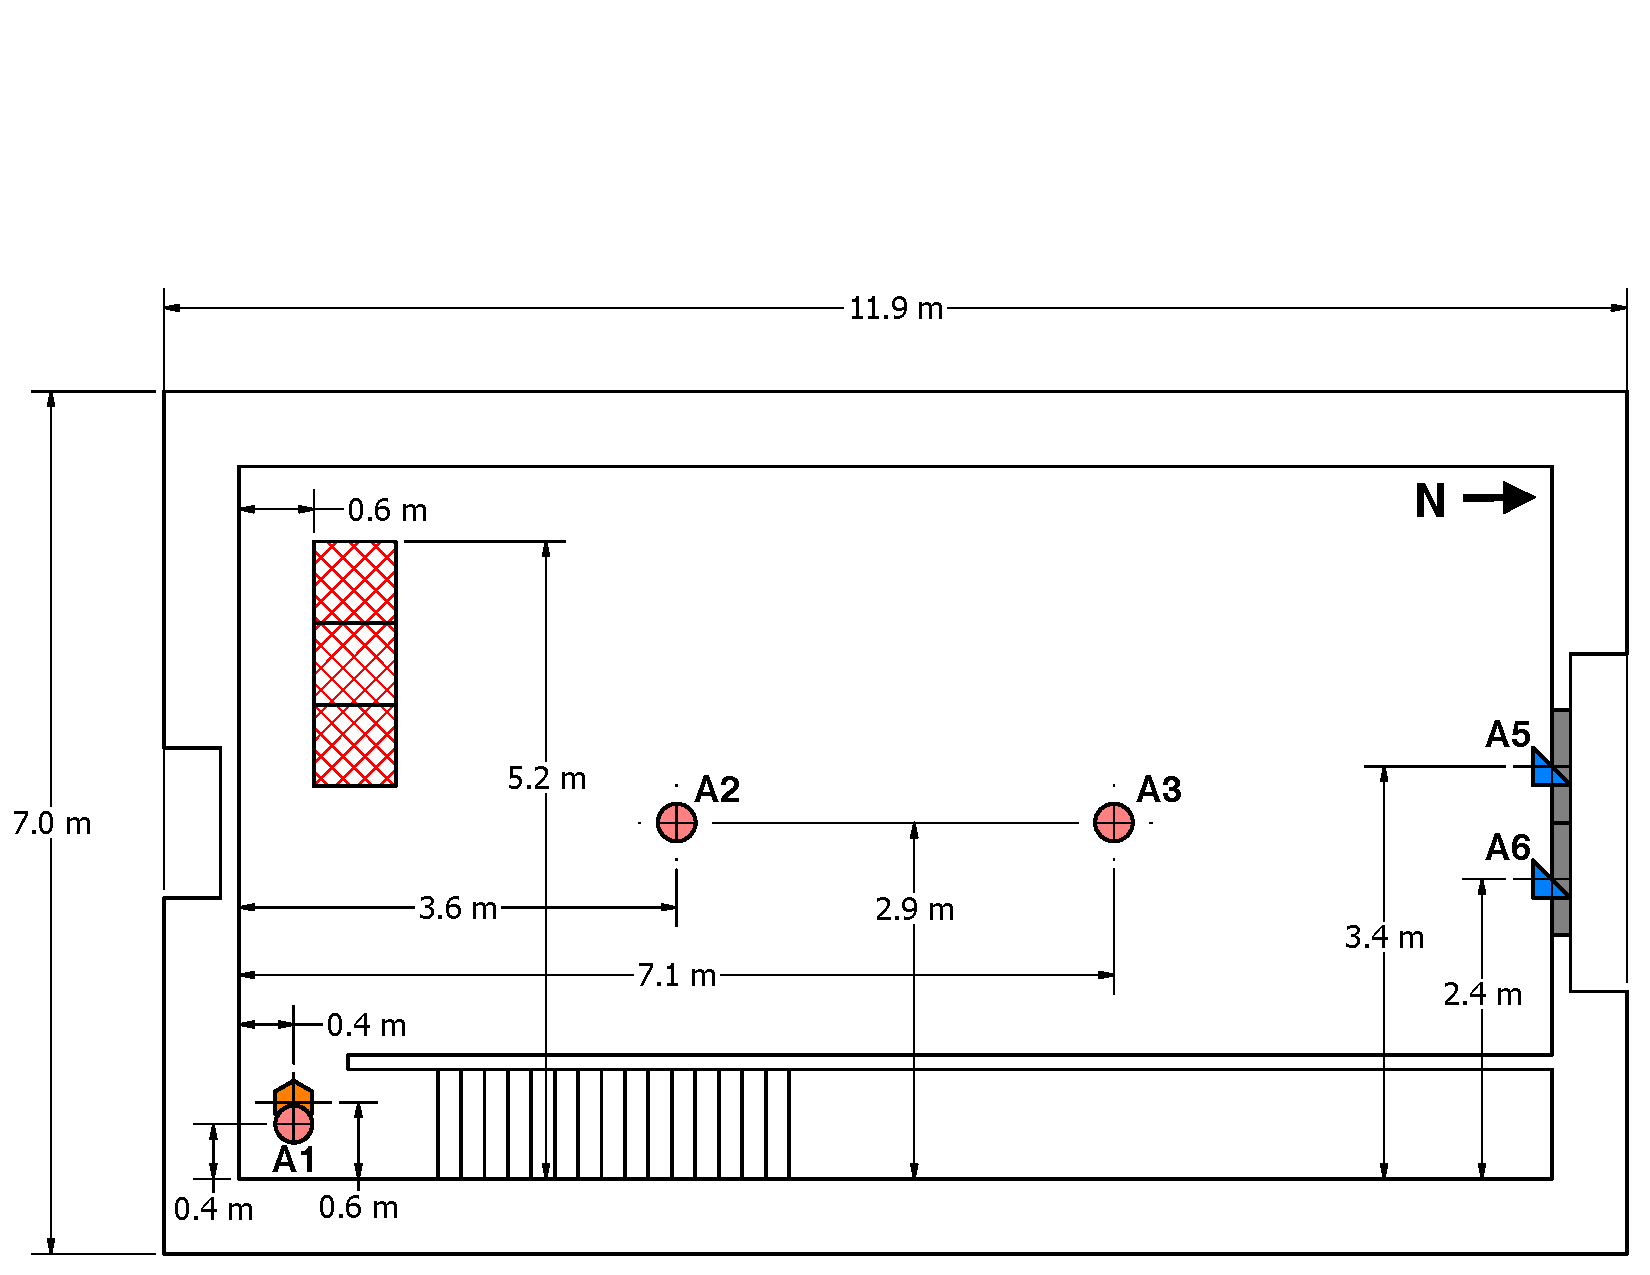
\includegraphics[width=\columnwidth]{Figures/Floor_Plans/West_Structure_1st_Floor_Dimensioned_Instrumentation}
	\caption[Locations and labels of instrumentation in the West Structure.]{Locations and labels of instrumentation in the second floor (top) and first floor (bottom) of the West Structure.}
	\label{fig:west_instrumentation}
\end{figure}

% \begin{figure}
% 	\centering
% 	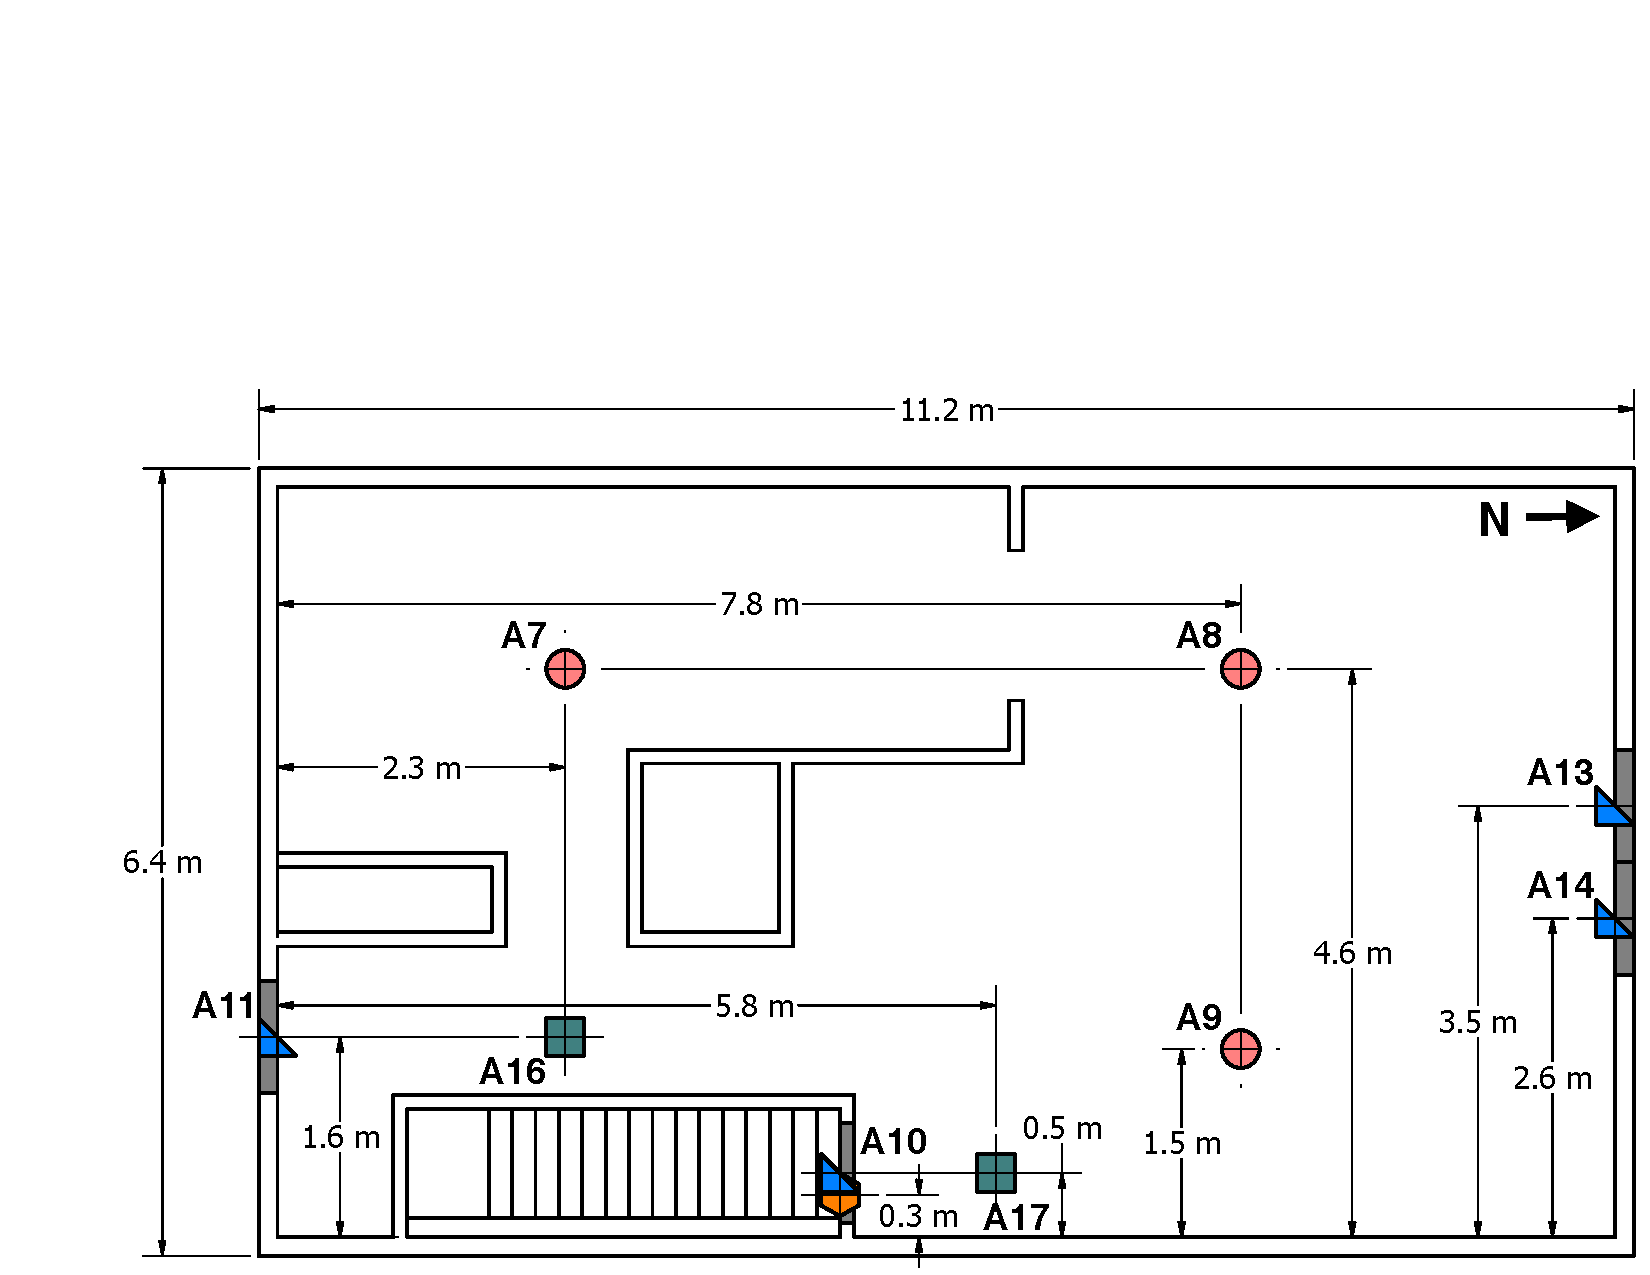
\includegraphics[width=0.94\columnwidth]{Figures/Floor_Plans/West_Structure_2nd_Floor_Dimensioned_Instrumentation}
% 	\\~\\
% 	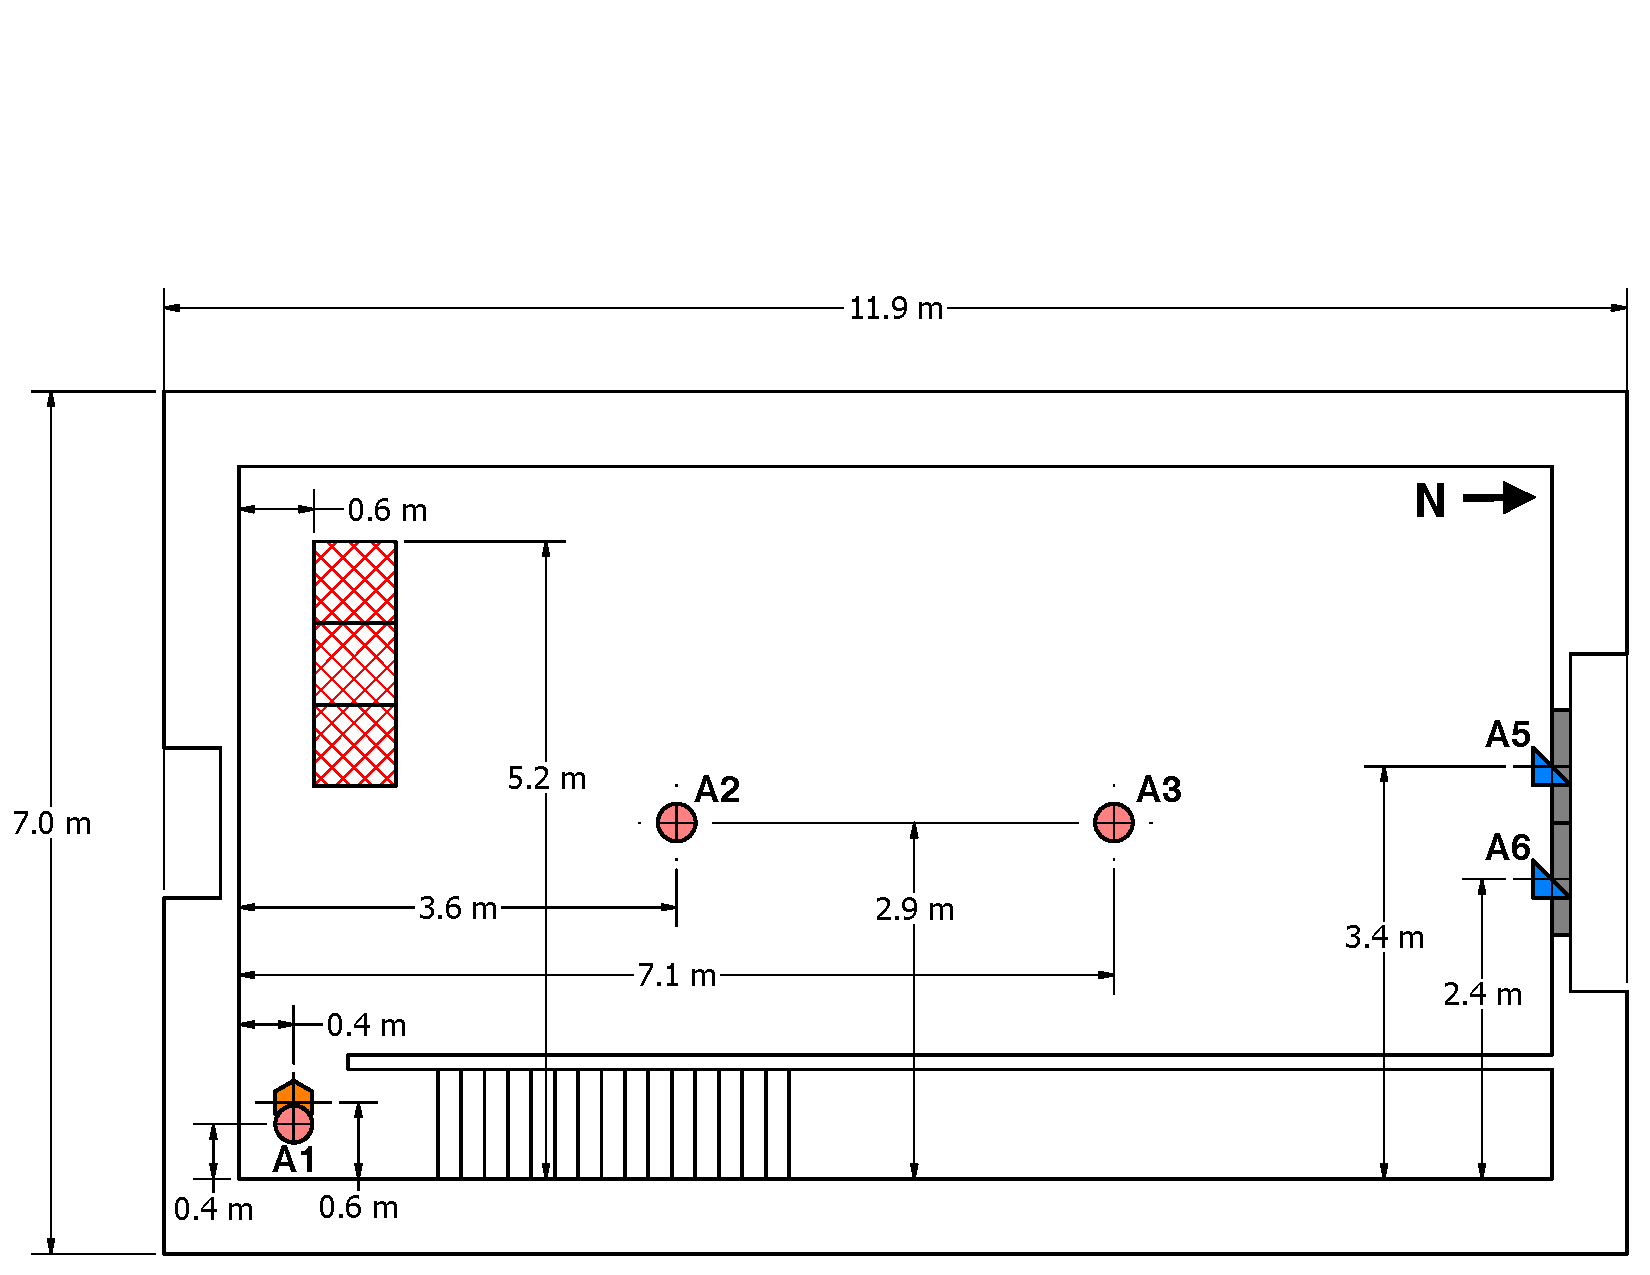
\includegraphics[width=\columnwidth]{Figures/Floor_Plans/West_Structure_1st_Floor_Dimensioned_Instrumentation}
% 	\caption[Locations and labels of instrumentation in the West Structure]{Locations and labels of instrumentation in the second floor (top) and first floor (bottom) of the West Structure.}
% 	\label{fig:west_instrumentation}
% \end{figure}

The thermocouple arrays and bi-directional probe plus solid thermocouple arrays contained eight sensors per array. Gas samples were pulled through 9.5~mm (0.38~in) diameter stainless steel tubing located 1.2~m (4~ft) above the floor. Each pair of total heat flux sensors was located 1.0~m (3.3~ft) above the floor. The pair at A16 contained one sensor facing the ceiling and another facing the north side of the room, and the pair at A17 contained one sensor facing the ceiling and another facing the stairway door. The height of each individual sensor in the sensor arrays is listed in the channel list found in Table~\ref{table:west_channel_list}.
\FloatBarrier

\subsection{Measurement Uncertainty}
This section lists the uncertainties in the reported length, mass, temperature, heat flux, gas species concentration, gas velocity, and heat release rate measurements. Uncertainty estimates are based either on manufacturer literature or analyses performed by others for similar measurement devices and techniques. In accordance with NIST guidelines~\cite{Taylor&Kuyatt:1994}, measurement accuracy is reported as an \textit{expanded uncertainty}, or 95~\% ($2\,\sigma$) confidence interval. Most manufacturer specifications express accuracy in terms of a \textit{standard  uncertainty}, or 68~\% ($1\,\sigma$) confidence interval.

\subsubsection*{\textit{Compartment Dimensions}}
Room dimensions and instrumentation location measurements were made with a hand held laser measurement device with a standard uncertainty of $\pm$6.0~mm (0.25~in) over a range of 0.6~m (2.0~ft) to 15~m (50.0~ft) according to the manufacturer~\cite{StanleyTools}. Steel measuring tapes with a resolution of $\pm$0.5~mm (0.02~in) were used to locate measurement devices. The steel measuring tapes were manufactured in compliance with NIST Manual 44~\cite{Butcher:2012}, which specifies a tolerance of $\pm$1.6~mm (0.06~in) for 9.1~m (30~ft) tapes and $\pm$6.4~mm (0.25~in) for 30.5~m (100~ft) tapes. These uncertainties are all well within the precision of the reported dimensions, which are typically rounded to the nearest 0.1~m.

\subsubsection*{\textit{Thermocouples}}
The standard uncertainty in the temperature of the thermocouple wire itself as stated by the wire manufacturer, OMEGA Engineering, Inc., is $\pm$2.2$~^{\circ}$C at $277~^{\circ}$C and increases to $\pm$9.5$~^{\circ}$C at $871~^{\circ}$C~\cite{Omega:2004}. The variation of the temperature in the environment surrounding the thermocouple is known to be much greater than that of the wire uncertainty. Expanded uncertainties as high as 20~\% for upper layer temperatures measured by a 1~mm bare-bead type K thermocouple have been reported by NIST researchers~\cite{Blevins:1999,Pitts:2003}. Small diameter thermocouples were used during these experiments to limit the impact of radiative heating and cooling. The estimated expanded uncertainty associated with the temperature measurements is $\pm$15~\%.

\subsubsection*{\textit{Heat Flux Gauges}}
Total heat flux measurements were made using water-cooled Schmidt-Boelter gauges. The manufacturer, MEDTHERM Corporation, reports a $\pm$3~\% calibration expanded uncertainty for these devices~\cite{Medtherm:2003}. Results from an international study on total heat flux gauge calibration and response demonstrated that the expanded uncertainty of a Schmidt-Boelter gauge is typically $\pm$8~\%~\cite{Pitts:2006}.

\subsubsection*{\textit{Gas Sampling}}
A gas sampling system from California Analytical Instruments, Inc. (model 602P) with a relative expanded uncertainty of $\pm$1~\% when compared to span gas volume fractions~\cite{Bundy:2007} was used to make gas concentration measurements. However, according to a study by Lock~et~al.~\cite{Lock:1}, the non-uniformity and movement of exhaust gases contribute to an estimated expanded uncertainty of $\pm$12~\%.

\subsubsection*{\textit{Bi-Directional Probes}}
Bi-directional probes with Setra 264 pressure transducers from Setra Systems, Inc. were used to measure gas velocity through doorways. An expanded uncertainty ranging from $\pm$14~\% to $\pm$22~\% for bi-directional probes of similar design was calculated by Bryant of NIST~\cite{Bryant:FSJ2009}.

\subsubsection*{\textit{Heat Release Rate}}
A positive displacement rotary gas meter was used to measure the volume flow rate of propane into the gas burners. The manufacturer, Romet Limited, reports a relative standard uncertainty of $\pm$2~\% for this type of meter (model RM-3000)~\cite{Romet:2014}. A volumetric flow rate was calculated from the gas meter volume readings and used in conjunction with the heat of combustion of propane to calculate the heat release rate of the fire for each experiment. The total expanded uncertainty for the heat release rate obtained from this method is estimated to be $\pm8$~\%.